\documentclass[11pt,a4paper]{article}
\usepackage[margin=2.2cm]{geometry}
\usepackage[T1]{fontenc}
\usepackage{lmodern}
\usepackage{microtype}
\usepackage{amsmath,amssymb,amsthm,mathtools}
\usepackage{braket}
\usepackage{graphicx}
\usepackage{booktabs,multirow}
\usepackage{xcolor}
\usepackage[most]{tcolorbox}
\usepackage{enumitem}
\usepackage{tikz}
\usetikzlibrary{arrows.meta,positioning,shapes,fit,calc}
\usepackage{caption}
\usepackage{float}
\usepackage{listings}
\usepackage{titlesec}
\usepackage{fancyhdr}
\usepackage[colorlinks=true,linkcolor=blue!50!black,urlcolor=blue!50!black,citecolor=blue!50!black]{hyperref}
\usepackage{cleveref}

\definecolor{ink}{HTML}{1F4E79}
\definecolor{warn}{HTML}{C0392B}
\definecolor{good}{HTML}{1E8449}
\definecolor{note}{HTML}{B9770E}
\titleformat{\section}{\Large\bfseries\color{ink}}{\thesection}{0.6em}{}
\titleformat{\subsection}{\large\bfseries\color{ink}}{\thesubsection}{0.6em}{}
\pagestyle{fancy}\fancyhf{}
\lhead{\small Study notes -- Optimization Driven Quantum Circuit Reduction}
\rhead{\small arXiv:2502.14715}\cfoot{\thepage}

\newtcolorbox{intuition}[1][]{colback=blue!3,colframe=ink,fonttitle=\bfseries,title=Intuition,#1}
\newtcolorbox{example}[1][]{colback=green!3,colframe=good,fonttitle=\bfseries,title=Worked example,#1}
\newtcolorbox{careful}[1][]{colback=red!3,colframe=warn,fonttitle=\bfseries,title=Careful / what the paper does not say,#1}
\newtcolorbox{beyond}[1][]{colback=orange!4,colframe=note,fonttitle=\bfseries,title=Beyond the paper (verified by us),#1}
\newtcolorbox{tldr}{colback=ink!6,colframe=ink,fonttitle=\bfseries\large,title=The paper in one page}

\lstset{basicstyle=\ttfamily\small,columns=fullflexible,frame=single,backgroundcolor=\color{black!3},
  keywordstyle=\bfseries\color{ink},commentstyle=\itshape\color{black!55},mathescape=true,
  morekeywords={for,while,if,then,else,return,with,probability,loop,until,break}}

\newcommand{\RX}{\mathrm{RX}}\newcommand{\RY}{\mathrm{RY}}\newcommand{\RZ}{\mathrm{RZ}}
\newcommand{\RXX}{\mathrm{RXX}}\newcommand{\CZ}{\mathrm{CZ}}\newcommand{\CNOT}{\mathrm{CNOT}}

% tiny circuit-drawing helpers in plain TikZ
\newcommand{\gbox}[3]{\node[draw,fill=black!4,minimum width=8mm,minimum height=6mm,font=\scriptsize,align=center] at (#1,#2) {#3};}

\begin{document}

\begin{titlepage}
\centering
\vspace*{2cm}
{\Huge\bfseries\color{ink} Optimization Driven\\[4pt] Quantum Circuit Reduction}\\[10pt]
{\Large Complete study notes}\\[18pt]
{\large B.\ Rosenhahn, T.\,J.\ Osborne, C.\ Hirche (Leibniz Universit\"at Hannover)}\\[4pt]
arXiv:2502.14715v1 [quant-ph], 20 Feb 2025 \quad (published: New J.\ Phys.\ \textbf{27}, 104509 (2025))\\[30pt]
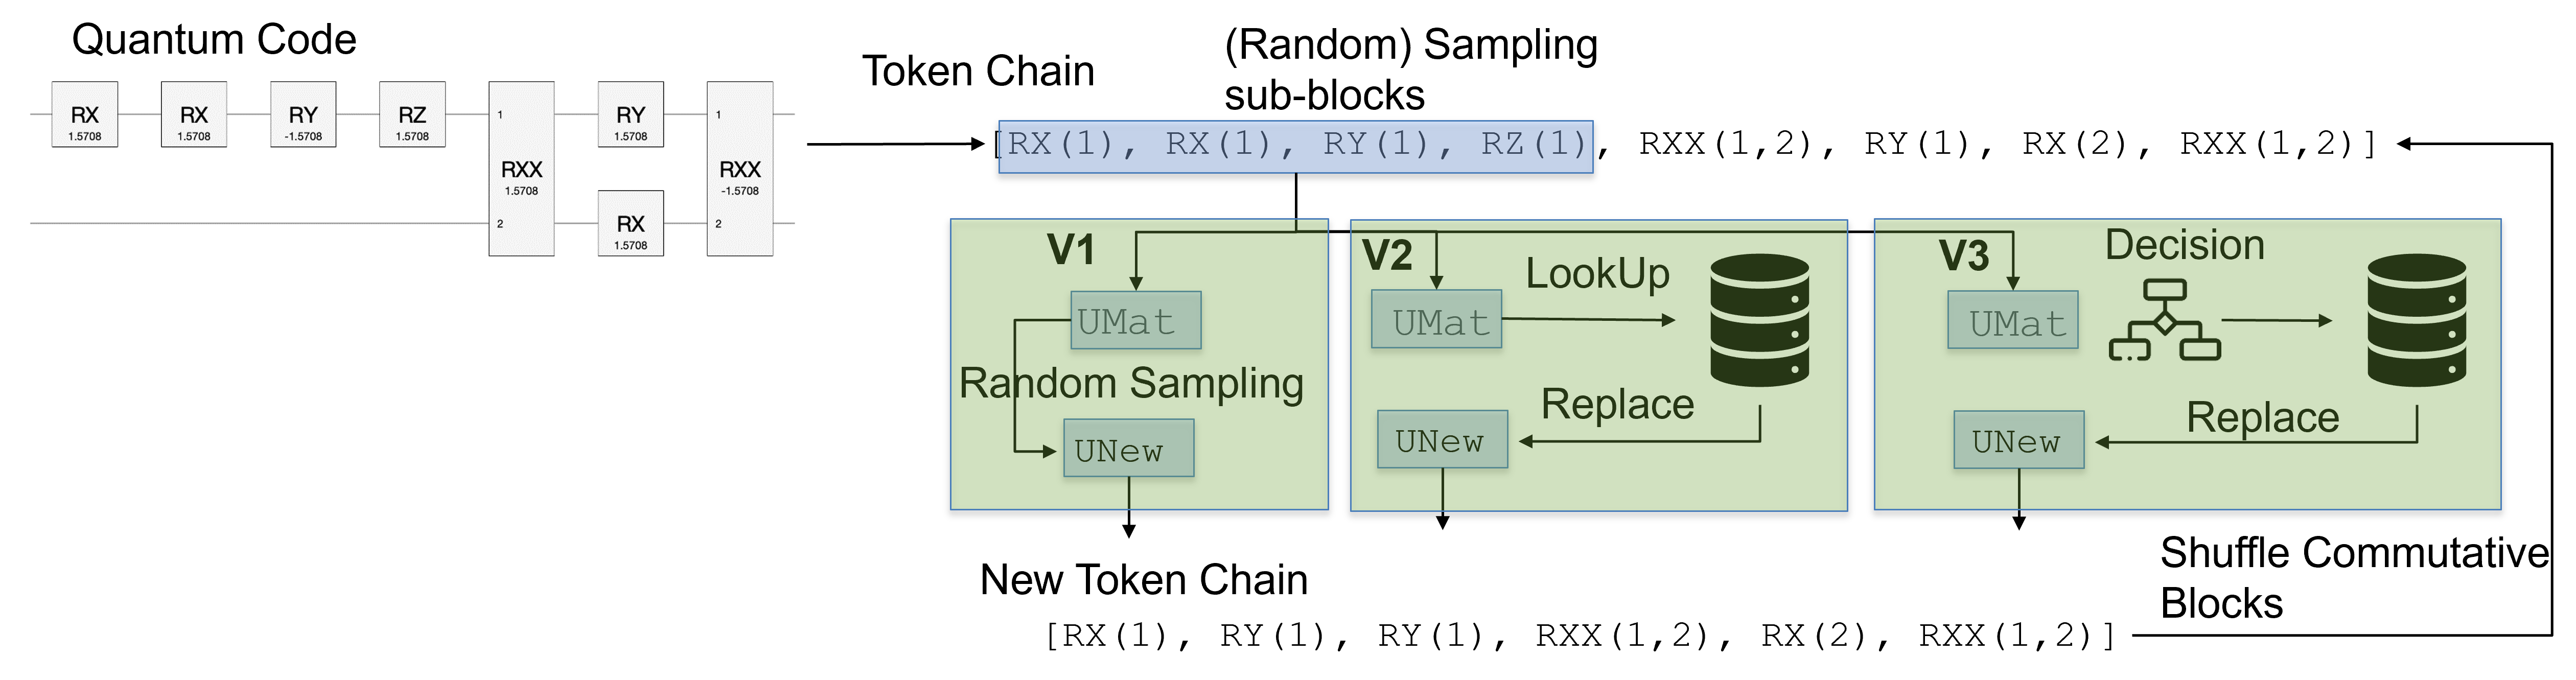
\includegraphics[width=\textwidth]{optVariantsW.png}\\[8pt]
{\small Figure 3 of the paper: the whole method in one picture.}\\[30pt]
\begin{minipage}{0.85\textwidth}\small
\textbf{How to use these notes.} Section~1 is a one-page summary. Section~2 teaches every piece of
background the paper assumes, from scratch (qubits, gates, global phase, commutation, compute graphs, random forests,
and the Clifford group, which the paper never names but which explains almost everything).
Sections~3--7 go through the paper in its own order, figure by figure and table by table, and say what each one
shows, how to read it, and what to watch out for. Section~8 explains the authors' MATLAB code line by line and
lists every place where code and paper disagree. Section~9 lists the changes in the published (NJP) version.
Section~10 is a critical assessment, Section~11 summarises whether each result reproduces, and Section~12 is a list of
exam/discussion questions with answers.
Every number marked \emph{verified} was recomputed by us with the reproduction code shipped alongside these notes.
\end{minipage}
\end{titlepage}

\tableofcontents
\newpage

%=====================================================================
\section{The paper in one page}
\begin{tldr}
\textbf{Problem.} A quantum computer can only execute a small \emph{native gate set}
(e.g.\ ion traps: $\RX,\RY,\RZ$ rotations and the two-qubit $\RXX$ gate; IBM: $\RX,\RZ$ and $\CZ$/$\CNOT$).
Translating a circuit into native gates gate-by-gate produces long, redundant circuits. Every extra gate adds noise
(decoherence), so we want the \emph{shortest circuit implementing exactly the same unitary matrix}.

\textbf{Idea.} Treat the circuit as a string of tokens (one token per gate), like a word in a formal language.
Repeatedly (1) pick a short random substring (2--8 gates), (2) compute the unitary it implements, (3) find a
\emph{shorter} string of native gates with the same unitary (up to a global phase), and (4) splice it in.
Between steps, randomly swap neighbouring gates that commute, so new substrings become reachable.

\textbf{Three ways to do step (3).}
\begin{itemize}[nosep]
\item \textbf{V1-RS (random sampling):} guess random shorter gate strings until one matches.
\item \textbf{V2-DR (database retrieval):} precompute a \emph{compute graph}: all unitaries reachable with at most
  $d$ gates (e.g.\ $d=4$), each stored with its shortest gate string. Step (3) becomes a database lookup.
\item \textbf{V3-RF (random forest):} a small classifier first predicts whether the substring is reducible at all,
  and only then is the (slow) lookup done.
\end{itemize}
\textbf{Scaling to many qubits.} A short substring touches only a few wires. Drop the idle wires, optimise on
$\le 3$ qubits, then map the result back (``wire reduction / wire lift'').

\textbf{Main results.} (i) Full compute graphs for 2 qubits (14 gates, depth $\le 6$) and 3 qubits (24 gates, depth $\le 5$)
(Table I). (ii) On 100 random circuits of length 100, mean time to reach a target length is
V1: 199\,s, V2: 55\,s, V3: 38\,s (Table II). (iii) Reduced circuits are far shorter than Qiskit's optimisation
levels 1--3: e.g.\ 300 ion-trap gates $\to$ Qiskit-L3 176, \emph{ours} 45 (Tables III--V). (iv) On IBM hardware, a
2-qubit circuit of 40 gates and its 8-gate equivalent give measurably different outcome distributions; the short
one is closer to the ideal simulation (Fig.~9).

\textbf{Main caveats} (details in \S10). Every gate the paper uses is a \emph{Clifford} gate, so all circuits live in
a \emph{finite} group. The problem therefore has exact, efficient solutions the paper does not use or compare against.
Benchmarks are on random circuits with single runs. The ``hardware'' experiment is one circuit, without error bars.
The released code has bugs that also show up in the paper's own figures.
\end{tldr}

%=====================================================================
\section{Background you need (from zero)}
\subsection{Qubits, registers and unitaries}
A qubit's state is a unit vector $\ket{\psi}=\alpha\ket0+\beta\ket1\in\mathbb C^2$. A register of $N$ qubits lives in
$\mathcal H=(\mathbb C^2)^{\otimes N}\cong\mathbb C^{2^N}$, so an $N$-qubit state has $2^N$ complex amplitudes. A
\textbf{gate} on $N$ qubits is a $2^N\times2^N$ unitary matrix $U$ ($U^\dagger U=I$). A gate acting on a subset of qubits
is extended to the whole register by tensoring with identities: e.g.\ a single-qubit gate $G$ on qubit 2 of 3 is
$I\otimes G\otimes I$.

\textbf{Circuits are products, read right-to-left.} A circuit (gate list) $(O(1),O(2),\dots,O(L))$, where $O(1)$ is
applied \emph{first}, implements
\[
U = O(L)\,O(L-1)\cdots O(1)\qquad\text{(paper Eq.~1)}.
\]
The first gate in time is the right-most matrix. Every ``token chain'' in the paper is written in this
right-to-left order.

\subsection{The gates used in the paper}
With the Pauli matrices $X=\begin{psmallmatrix}0&1\\1&0\end{psmallmatrix}$, $Y=\begin{psmallmatrix}0&-i\\i&0\end{psmallmatrix}$,
$Z=\begin{psmallmatrix}1&0\\0&-1\end{psmallmatrix}$:
\begin{gather*}
\RX(\theta)=e^{-i\theta X/2}=\begin{pmatrix}\cos\frac\theta2&-i\sin\frac\theta2\\-i\sin\frac\theta2&\cos\frac\theta2\end{pmatrix},\\
\RY(\theta)=\begin{pmatrix}\cos\frac\theta2&-\sin\frac\theta2\\\sin\frac\theta2&\cos\frac\theta2\end{pmatrix},\quad
\RZ(\theta)=\begin{pmatrix}e^{-i\theta/2}&0\\0&e^{i\theta/2}\end{pmatrix}.
\end{gather*}
Geometrically, $\RX(\theta)$ rotates the Bloch sphere by angle $\theta$ about the $x$ axis, and so on. The two-qubit gates are
\begin{gather*}
\RXX(\theta)=e^{-i\theta\,X\otimes X/2}=\cos\tfrac\theta2\,I-i\sin\tfrac\theta2\,X\otimes X,\\
\CZ=\mathrm{diag}(1,1,1,-1),\qquad \CNOT=\ket0\!\bra0\otimes I+\ket1\!\bra1\otimes X.
\end{gather*}
$\RXX(\pi/2)$ is the M{\o}lmer--S{\o}rensen gate, the native entangling gate of trapped-ion machines.
$\CZ$/$\CNOT$/ECR play that role on IBM superconducting chips. $H=\frac1{\sqrt2}\begin{psmallmatrix}1&1\\1&-1\end{psmallmatrix}$
(Hadamard) appears in the Bell example.

\textbf{Discretised angles.} The paper (and its code) only uses $\theta\in\{-\pi/2,+\pi/2\}$ for rotations and
$\RXX(\pm\pi/2)$. So the ``gate set'' is a finite list. For $n$ qubits the ion-trap list has $6n$ single-qubit gates
(3 axes $\times$ 2 signs $\times$ $n$ qubits) plus one or two $\RXX$ per qubit pair. The paper's operator counts
come from this: $n=2$: $12+2=14$; $n=3$: $18+6=24$ (Table~I). These counts use $\RXX(\pm\pi/2)$; the demo code uses only
$\RXX(+\pi/2)$, giving 13 and 21.

\subsection{Global phase: why ``equal up to a phase''}
Two unitaries $U$ and $e^{i\varphi}U$ produce the same measurement statistics for every input, because the phase cancels
in $|\braket{x|U|\psi}|^2$. So the paper compares circuits \emph{up to global phase}, with a numerical tolerance
($10^{-5}$ in the text, $10^{-3}$ in the code). The code (\texttt{compare.m}) finds the best complex scale
$s=\frac{\langle R,F\rangle}{\langle R,R\rangle}$ by least squares and returns $\|sR-F\|_2$.
\begin{example}
$\RZ(\pi/2)=\mathrm{diag}(e^{-i\pi/4},e^{i\pi/4})=e^{-i\pi/4}\,\mathrm{diag}(1,i)=e^{-i\pi/4}S$. So the phase gate $S$ and
$\RZ(\pi/2)$ are ``the same gate'' for this paper. Likewise $\RX(\pi/2)^2=\RX(\pi)=-iX\simeq X$.
\end{example}

\subsection{Commuting gates and why the method shuffles}
Gates $A,B$ commute if $AB=BA$; then the order of two neighbouring tokens can be swapped without changing the circuit.
Typical cases: gates on disjoint qubits; $\RZ$ on either qubit of a $\CZ$ (both diagonal); $\RX$ on either qubit
of an $\RXX$ ($X\otimes I$ commutes with $X\otimes X$). Swapping commuting neighbours changes which gates are
\emph{adjacent}, and so which substrings the local optimiser can see. Example: in $\RZ_1\,\CZ_{12}\,\RZ_1^{-1}$
the two $\RZ$s cancel only after $\RZ_1$ is moved across the $\CZ$. The paper's code tests commutation numerically,
for each adjacent pair.

\subsection{Transpilation, QAS and QAM vocabulary}
\begin{itemize}[nosep]
\item \textbf{Transpilation}: rewriting a circuit for specific hardware (native gates + qubit connectivity).
\item \textbf{QAS} (quantum architecture search): automatic search for a circuit implementing a target
  (named after neural architecture search in ML).
\item \textbf{QAM} (quantum architecture mapping): the four sub-problems (a) gate synthesis (translate to native gates),
  (b) mapping/routing (respect connectivity, insert SWAPs), (c) gate optimisation (shorten), (d) resource allocation.
  \textbf{This paper only addresses (c)}: it assumes a correct native-gate circuit is given and shortens it.
\item \textbf{Decoherence}: loss of quantum information to the environment over time. Longer circuits accumulate more error.
\item \textbf{Quantum volume}: a hardware benchmark built from random square circuits. Shorter compiled circuits score better.
\item \textbf{EPLG} (error per layered gate) and \textbf{CLOPS} (circuit layer operations per second): IBM's
  error and speed metrics, quoted in the hardware section.
\end{itemize}

\subsection{The Clifford group (not named in the paper, but essential)}\label{sec:clifford}
\begin{beyond}
A \emph{Clifford} unitary maps every Pauli string (e.g.\ $X\otimes Z$) to $\pm$ another Pauli string under conjugation.
Rotations by $\pm\pi/2$ about $x,y,z$, $\RXX(\pm\pi/2)$, $\CZ$, $\CNOT$ and $H$ are all Clifford. Products of Cliffords are
Clifford. So \textbf{every circuit in this paper is an element of the Clifford group}. Modulo global phase this group is
\emph{finite}:
\[
|\mathcal C_n/U(1)| = 2^{n^2+2n}\prod_{j=1}^n(4^j-1):\qquad
|\mathcal C_1|=24,\quad |\mathcal C_2|=11{,}520,\quad |\mathcal C_3|=92{,}897{,}280 .
\]
Consequences used throughout these notes:
\begin{enumerate}[nosep]
\item The compute graph of the paper is a ball in the \emph{Cayley graph} of this finite group (nodes = group elements,
  edges = multiplication by a generator). Grown far enough, it \emph{stops growing}. For 2 qubits with the 14 ion-trap
  gates it saturates at depth 10 with all 11,520 elements (Fig.~\ref{fig:growth}).
\item Therefore \textbf{any 2-qubit circuit over these gates, however long, has an equivalent with at most 10 gates}
  (13-gate pool: also 10; IBM $\RX,\RZ,\CZ$ pool: 11). A random 2-qubit circuit needs about 6 on average (verified).
\item A Clifford is determined exactly by a small binary ``tableau'' (where it sends $X_i,Z_i$), so equality can be checked
  exactly with integers instead of with a floating-point tolerance (Gottesman--Knill / Aaronson--Gottesman).
\end{enumerate}
\end{beyond}
\begin{figure}[H]\centering
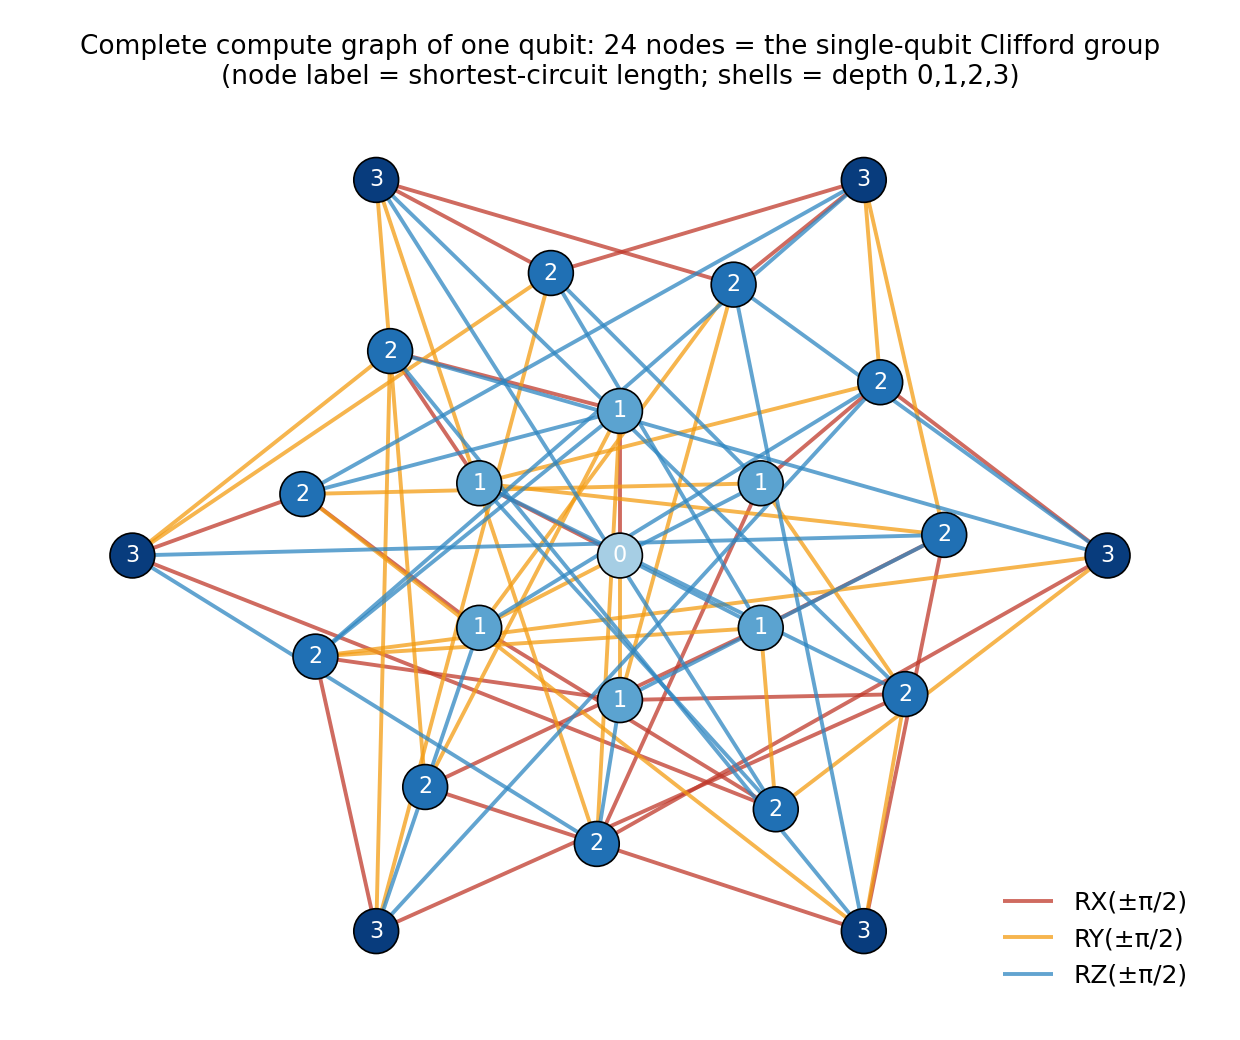
\includegraphics[width=0.62\textwidth]{notes_1q_graph.png}
\caption{(Ours.) The full compute graph for one qubit with gates $\RX,\RY,\RZ(\pm\pi/2)$. It has exactly 24 nodes:
the single-qubit Clifford group. Every single-qubit circuit over these gates is equal (up to phase) to one with
at most 3 gates.}\label{fig:1q}
\end{figure}

\subsection{Decision trees and random forests (needed for V3)}
A decision tree classifies an input by a sequence of yes/no questions on its features. Each question (split) is chosen
to maximise the \textbf{information gain}, the drop in Shannon entropy
$H(T)=-\sum_i p_i\log_2p_i$ from the parent node to the (weighted) children:
\[IG(T,a)=H(T)-H(T\mid a).\]
\begin{example}
100 blocks, 30 reducible ($p=0.3$): $H=-0.3\log_20.3-0.7\log_20.7=0.881$ bits. A split on the feature ``block contains two
identical adjacent $\RX$'' sends 20 blocks left (18 reducible) and 80 right (12 reducible).
$H_{\text{left}}=H(0.9)=0.469$, $H_{\text{right}}=H(0.15)=0.610$, so $H(T|a)=0.2\cdot0.469+0.8\cdot0.610=0.582$ and
$IG=0.881-0.582=0.30$ bits. The tree picks the split with the largest $IG$.
\end{example}
A \textbf{random forest} trains many trees, each on a bootstrap sample of the data (``bagging'') and with random feature
subsets, and takes a majority vote. It is fast to train (paper: $<1$\,s) and very fast to evaluate (paper: $<10^{-4}$\,s).
\begin{careful}
The paper's displayed $IG$ formula is sloppy: the second sum should be the \emph{expectation over the values of $a$} of the
child entropies, $H(T|a)=\sum_v \Pr(a{=}v)\,H(T\mid a{=}v)$, not a single sum $\sum_i\Pr(i|a)\log\Pr(i|a)$. The paper also
never says what \emph{features} the forest sees, how many trees it has, or its accuracy. These details decide
whether V3 helps (see \S\ref{sec:v3}).
\end{careful}

%=====================================================================
\section{Paper \S I: Introduction and motivation}
The introduction argues that circuit length matters both below the fault-tolerance threshold (decoherence) and just above
it (each logical gate is expensive). It surveys QAS methods: Gibbs sampling, evolutionary/genetic algorithms, neural
predictors, gradient-based methods, MCTS, Monte Carlo \emph{Graph} Search (MCGS, the authors' earlier work [35,36]),
ranking, and RL. It also surveys QAM work (SWAP-insertion with SMT solvers, ion-trap QCCD shuttling).
The authors position this paper as \emph{circuit reduction}: they start from an existing mapping, whose length is an upper
bound, and shrink it with local term replacement.

\begin{figure}[H]\centering
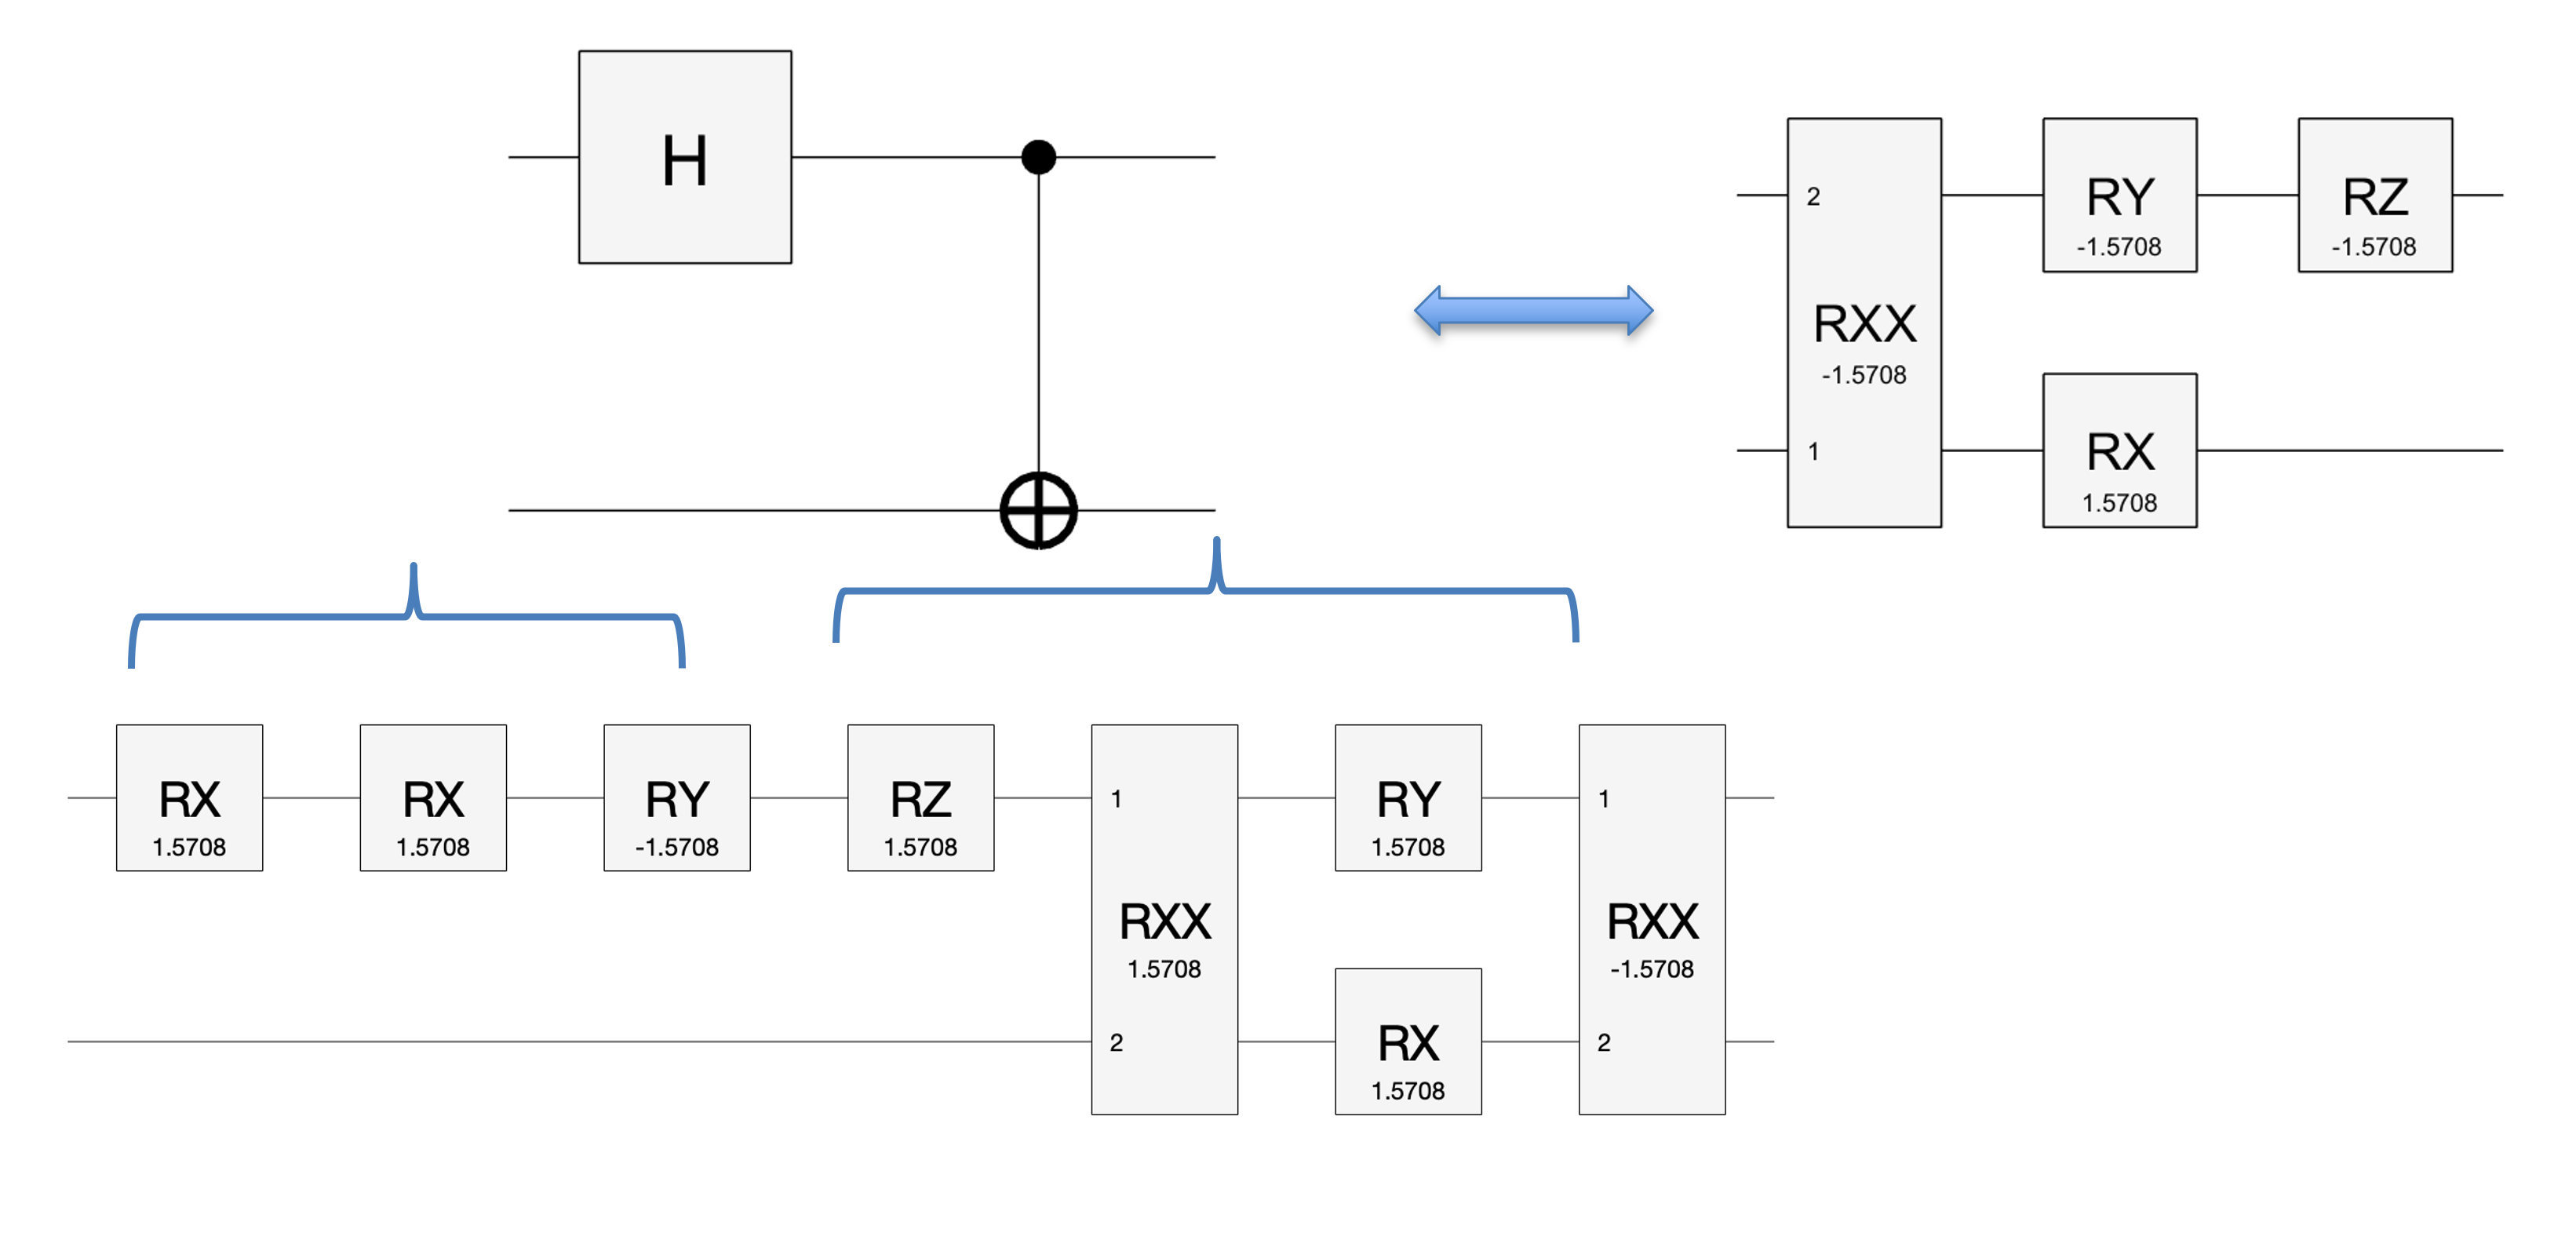
\includegraphics[width=0.75\textwidth]{Motivation1.png}
\caption{Paper Fig.~1. Top-left: Bell-state circuit ($H$ then $\CNOT$). Bottom: naive translation into ion-trap gates
(the $H$ becomes $\RX\,\RX\,\RY$, the $\CNOT$ becomes $\RZ,\RXX,\RY,\RX,\RXX$): 8 gates. Right: an equivalent 4-gate circuit.}
\end{figure}
\begin{example}[title=Worked example: checking Fig.~1 (verified)]
Bottom row (time order): $\RX_1(\tfrac\pi2),\RX_1(\tfrac\pi2),\RY_1(-\tfrac\pi2)$ $\big[\simeq H$ up to phase$\big]$, then
$\RZ_1(\tfrac\pi2),\RXX_{12}(\tfrac\pi2),\RY_1(\tfrac\pi2),\RX_2(\tfrac\pi2),\RXX_{12}(-\tfrac\pi2)$ $\big[\simeq\CNOT\big]$.
Right: $\RXX_{12}(-\tfrac\pi2)$, then $\RY_1(-\tfrac\pi2),\RZ_1(-\tfrac\pi2)$ on qubit 1 and $\RX_2(\tfrac\pi2)$ on qubit 2.
Multiplying the matrices, both equal $\CNOT\,(H\otimes I)$ up to global phase to $10^{-13}$. On $\ket{00}$ both give
$\propto(\ket{00}+\ket{11})/\sqrt2$. A full search over all 11,520 two-qubit Cliffords shows that \textbf{4 is optimal}: no
3-gate ion-trap circuit makes this unitary. $\CNOT$ alone needs 5 ion-trap gates.
\end{example}
\textbf{Karnaugh-map analogy.} In classical logic minimisation, Karnaugh maps arrange a truth table in Gray-code order
(neighbouring cells differ in one variable), so that groups of 1s can be merged into simpler terms. The paper mentions this
only as motivation: no direct quantum analogue exists, which is why they turn to search.

\textbf{Claimed contributions.} (1) V1-RS, (2) V2-DR, (3) V3-RF, (4) an IBM hardware evaluation, (5) code release.

%=====================================================================
\section{Paper \S II: Preliminaries}
\subsection{Token chains (\S II.A)}
Number the available gates $1,\dots,|\mathcal{OP}|$. A circuit is then a string of integers, its \emph{token chain}. This
turns circuit optimisation into \textbf{string rewriting}. In formal-language terms, a \emph{grammar} is a set of
rewriting rules ``replace substring $a$ by $b$''. The paper's rules are ``replace any substring by a shorter one with the
same unitary''. The rules are never written down; they are found on the fly (V1) or read from a database (V2/V3).

\subsection{Compute graphs (\S II.B, Table I, Fig.~2)}\label{sec:cg}
Start from the identity matrix (root). Apply every available gate to every current node. If the resulting unitary is
new (up to phase, within tolerance), create a node; otherwise add an edge to the existing node. Repeat to a fixed depth $d$.
The shortest path from the root to a node gives the \textbf{shortest circuit} for that node's unitary (among circuits of
length $\le d$). The paper stores (unitary, shortest circuit) pairs in a database for V2/V3.

\begin{figure}[H]\centering
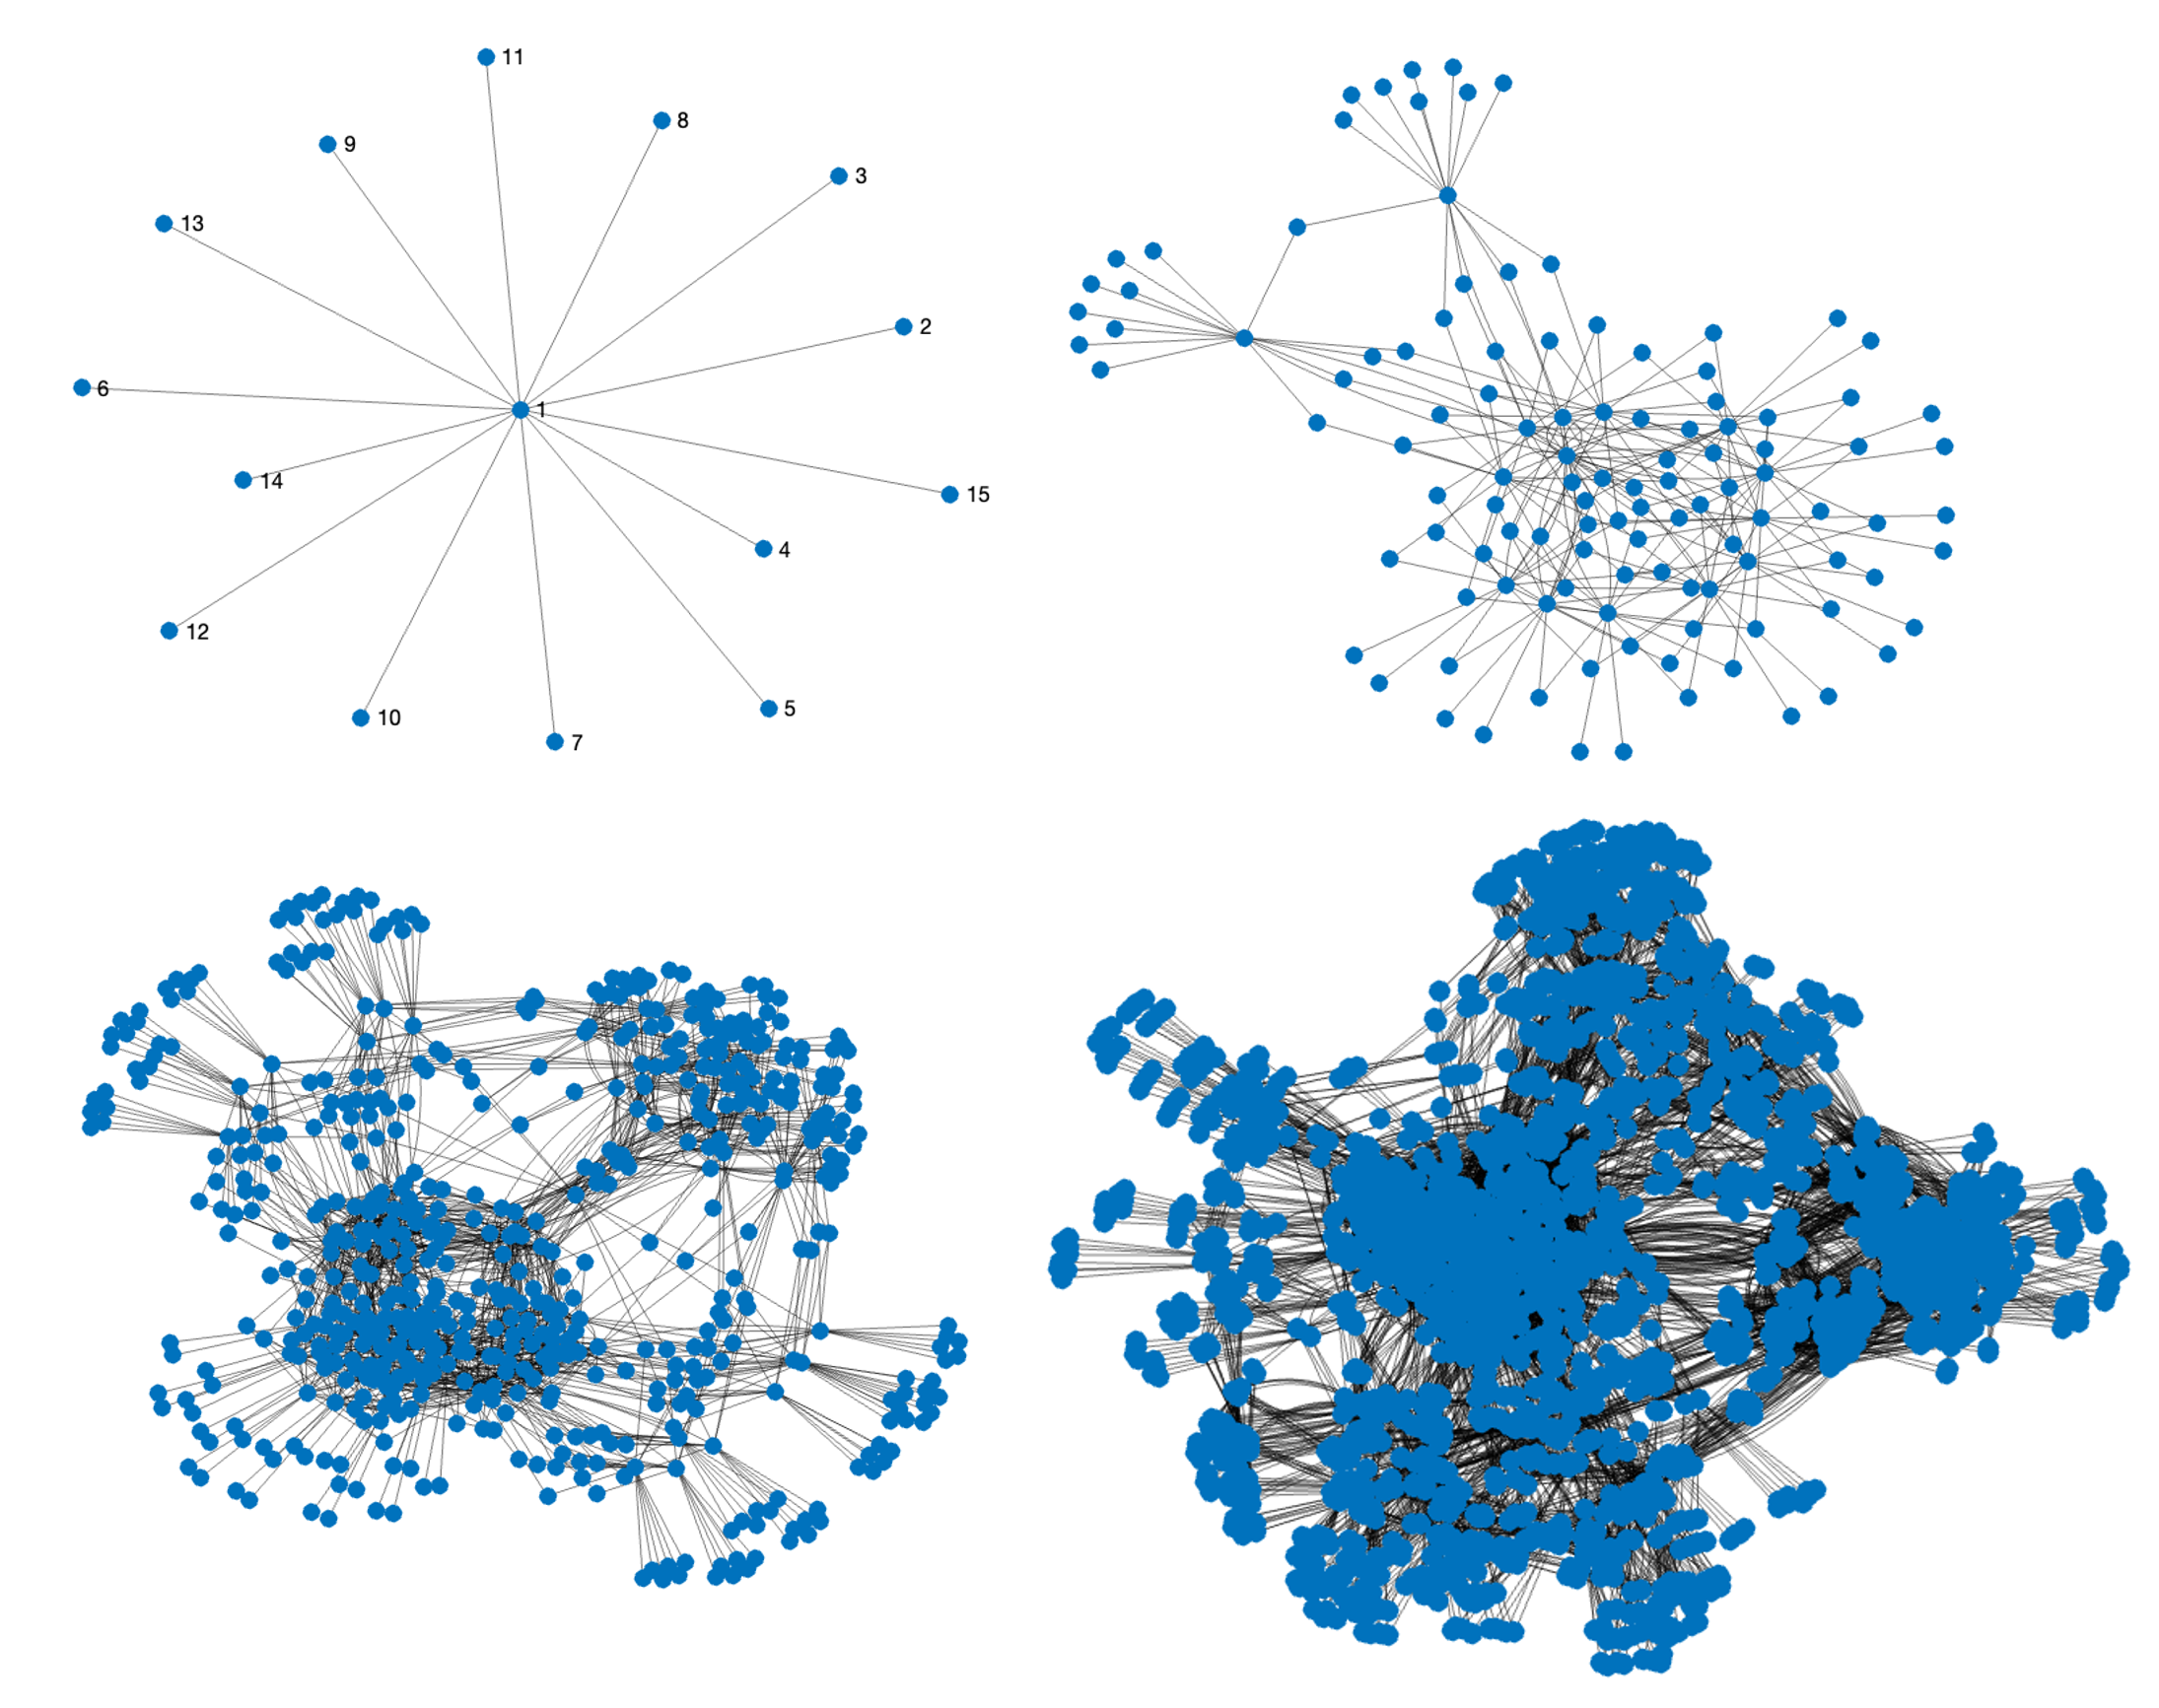
\includegraphics[width=0.62\textwidth]{FullComputeGraphs2.png}
\caption{Paper Fig.~2: compute graphs of depth 1, 2, 3, 4 for 14 operators (2 qubits). Depth 1 is a star (root + 14
children). Afterwards, many different gate strings land on the \emph{same} unitary, which creates cycles. That is why the
node count grows much more slowly than $14^d$.}
\end{figure}

\begin{table}[H]\centering
\begin{tabular}{ccc rr rr}\toprule
Qubits & \#Ops & Depth & Nodes (paper) & Edges (paper) & Nodes (ours) & $14^d$ or $24^d$\\\midrule
2&14&1&15&14&15 \checkmark&14\\
2&14&2&114&210&114 \checkmark&196\\
2&14&3&584&1{,}596&584 \checkmark&2{,}744\\
2&14&4&2{,}024&8{,}176&2{,}024 \checkmark&38{,}416\\
2&14&5&4{,}512&28{,}336&4{,}512 \checkmark&537{,}824\\
2&14&6&7{,}420&63{,}168&7{,}420 \checkmark&7.5\,M\\\midrule
3&24&1&25&24&25 \checkmark&24\\
3&24&2&337&600&337 \checkmark&576\\
3&24&3&3{,}215&8{,}088&3{,}215 \checkmark&13{,}824\\
3&24&4&23{,}622&77{,}160&23{,}622 \checkmark&331{,}776\\
3&24&5&137{,}572&566{,}928&137{,}572 \checkmark&8.0\,M\\\bottomrule
\end{tabular}
\caption{Paper Table I with our exact recomputation (Python, $<$5\,s in total).}
\end{table}
\begin{intuition}
\textbf{How to read Table I.} ``Nodes'' = number of distinct unitaries (up to phase) reachable with $\le d$ gates.
``Edges'' is \emph{not} the number of distinct arrows: the code adds one edge for every (node at distance $<d$, operator)
pair, including duplicates and self-loops, so $\text{Edges}(d)=\text{Nodes}(d-1)\times\#\text{Ops}$.
Check: $114\times14=1596$, $2024\times14=28336$, $23622\times24=566928$.
\end{intuition}
\begin{figure}[H]\centering
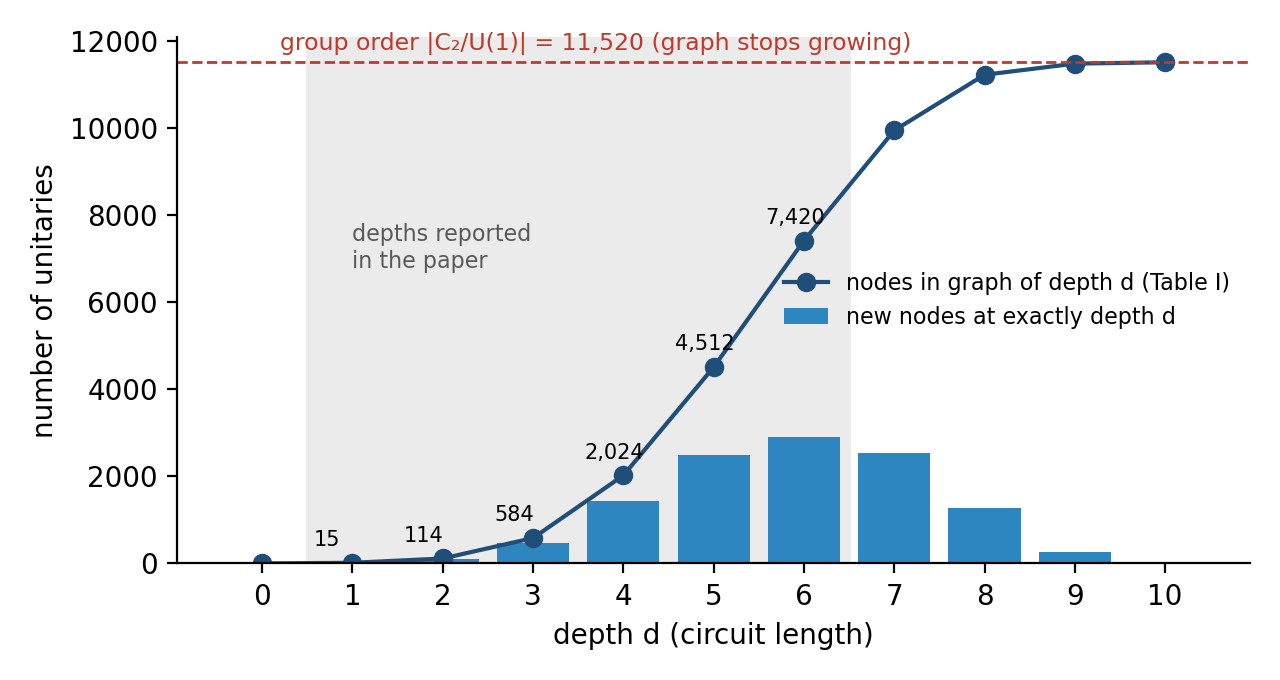
\includegraphics[width=0.75\textwidth]{notes_2q_growth.png}
\caption{(Ours.) Continuing Table I for 2 qubits beyond depth 6: the graph saturates at depth 10 with all 11,520 two-qubit
Cliffords. The paper's 2-qubit database (depth 6) holds 64\% of the group. A depth-10 database would hold all of it
and give the \emph{exact} optimum for any 2-qubit circuit with one lookup.}\label{fig:growth}
\end{figure}
\textbf{MCGS vs.\ full graph.} In their earlier MCGS work the graph was grown selectively, using Poisson/Gibbs-style
sampling to choose which node to expand. Here the graph is grown \emph{fully} to a fixed depth, which is feasible only for
small depth and few qubits.

\subsection{Random forests (\S II.C)}
See \S2.6 above. In the paper, a forest decides whether a sampled block is likely to be reducible before
the database is queried.

%=====================================================================
\section{Paper \S III: The three methods}
\subsection{The common loop}
\begin{lstlisting}
input: circuit g (token chain), pool of $\le$3-qubit gates, database DB (for V2/V3)
loop until |g| $\le$ target (or time budget):
    with probability 0.7: for each commuting adjacent pair, swap it with prob. 0.6
    pick start s uniformly, length $\ell=\min(\text{uniform},7)+1\in[2,8]$;
        resample until the block touches $\le$3 wires
    relabel the block's wires to 1..k ("wire reduction"), compute its $2^3\times2^3$ unitary $U_s$
    V1: draw random strings of p < $\ell$ pool gates until one has unitary $\simeq U_s$
    V2: look up $U_s$ in DB among entries of length < $\ell$
    V3: if RandomForest(block) says "reducible": do the V2 lookup, else skip
    if a shorter string w was found: map w back to the original wires ("wire lift"),
        replace the block by w, cancel adjacent inverse pairs (simplereduce)
\end{lstlisting}

\subsection{V1: random search}
Pick a random substring $U_s=O(m{+}n{-}1)\cdots O(m)$. Sample random shorter strings $U_p=O^r(p)\cdots O^r(1)$, $p<n$.
If $U_p\simeq U_s$, replace. Its weakness: two nested random processes (which block, and which candidate), and the chance
of hitting the right candidate shrinks like $|\mathcal{OP}|^{-p}$.

\begin{figure}[H]\centering
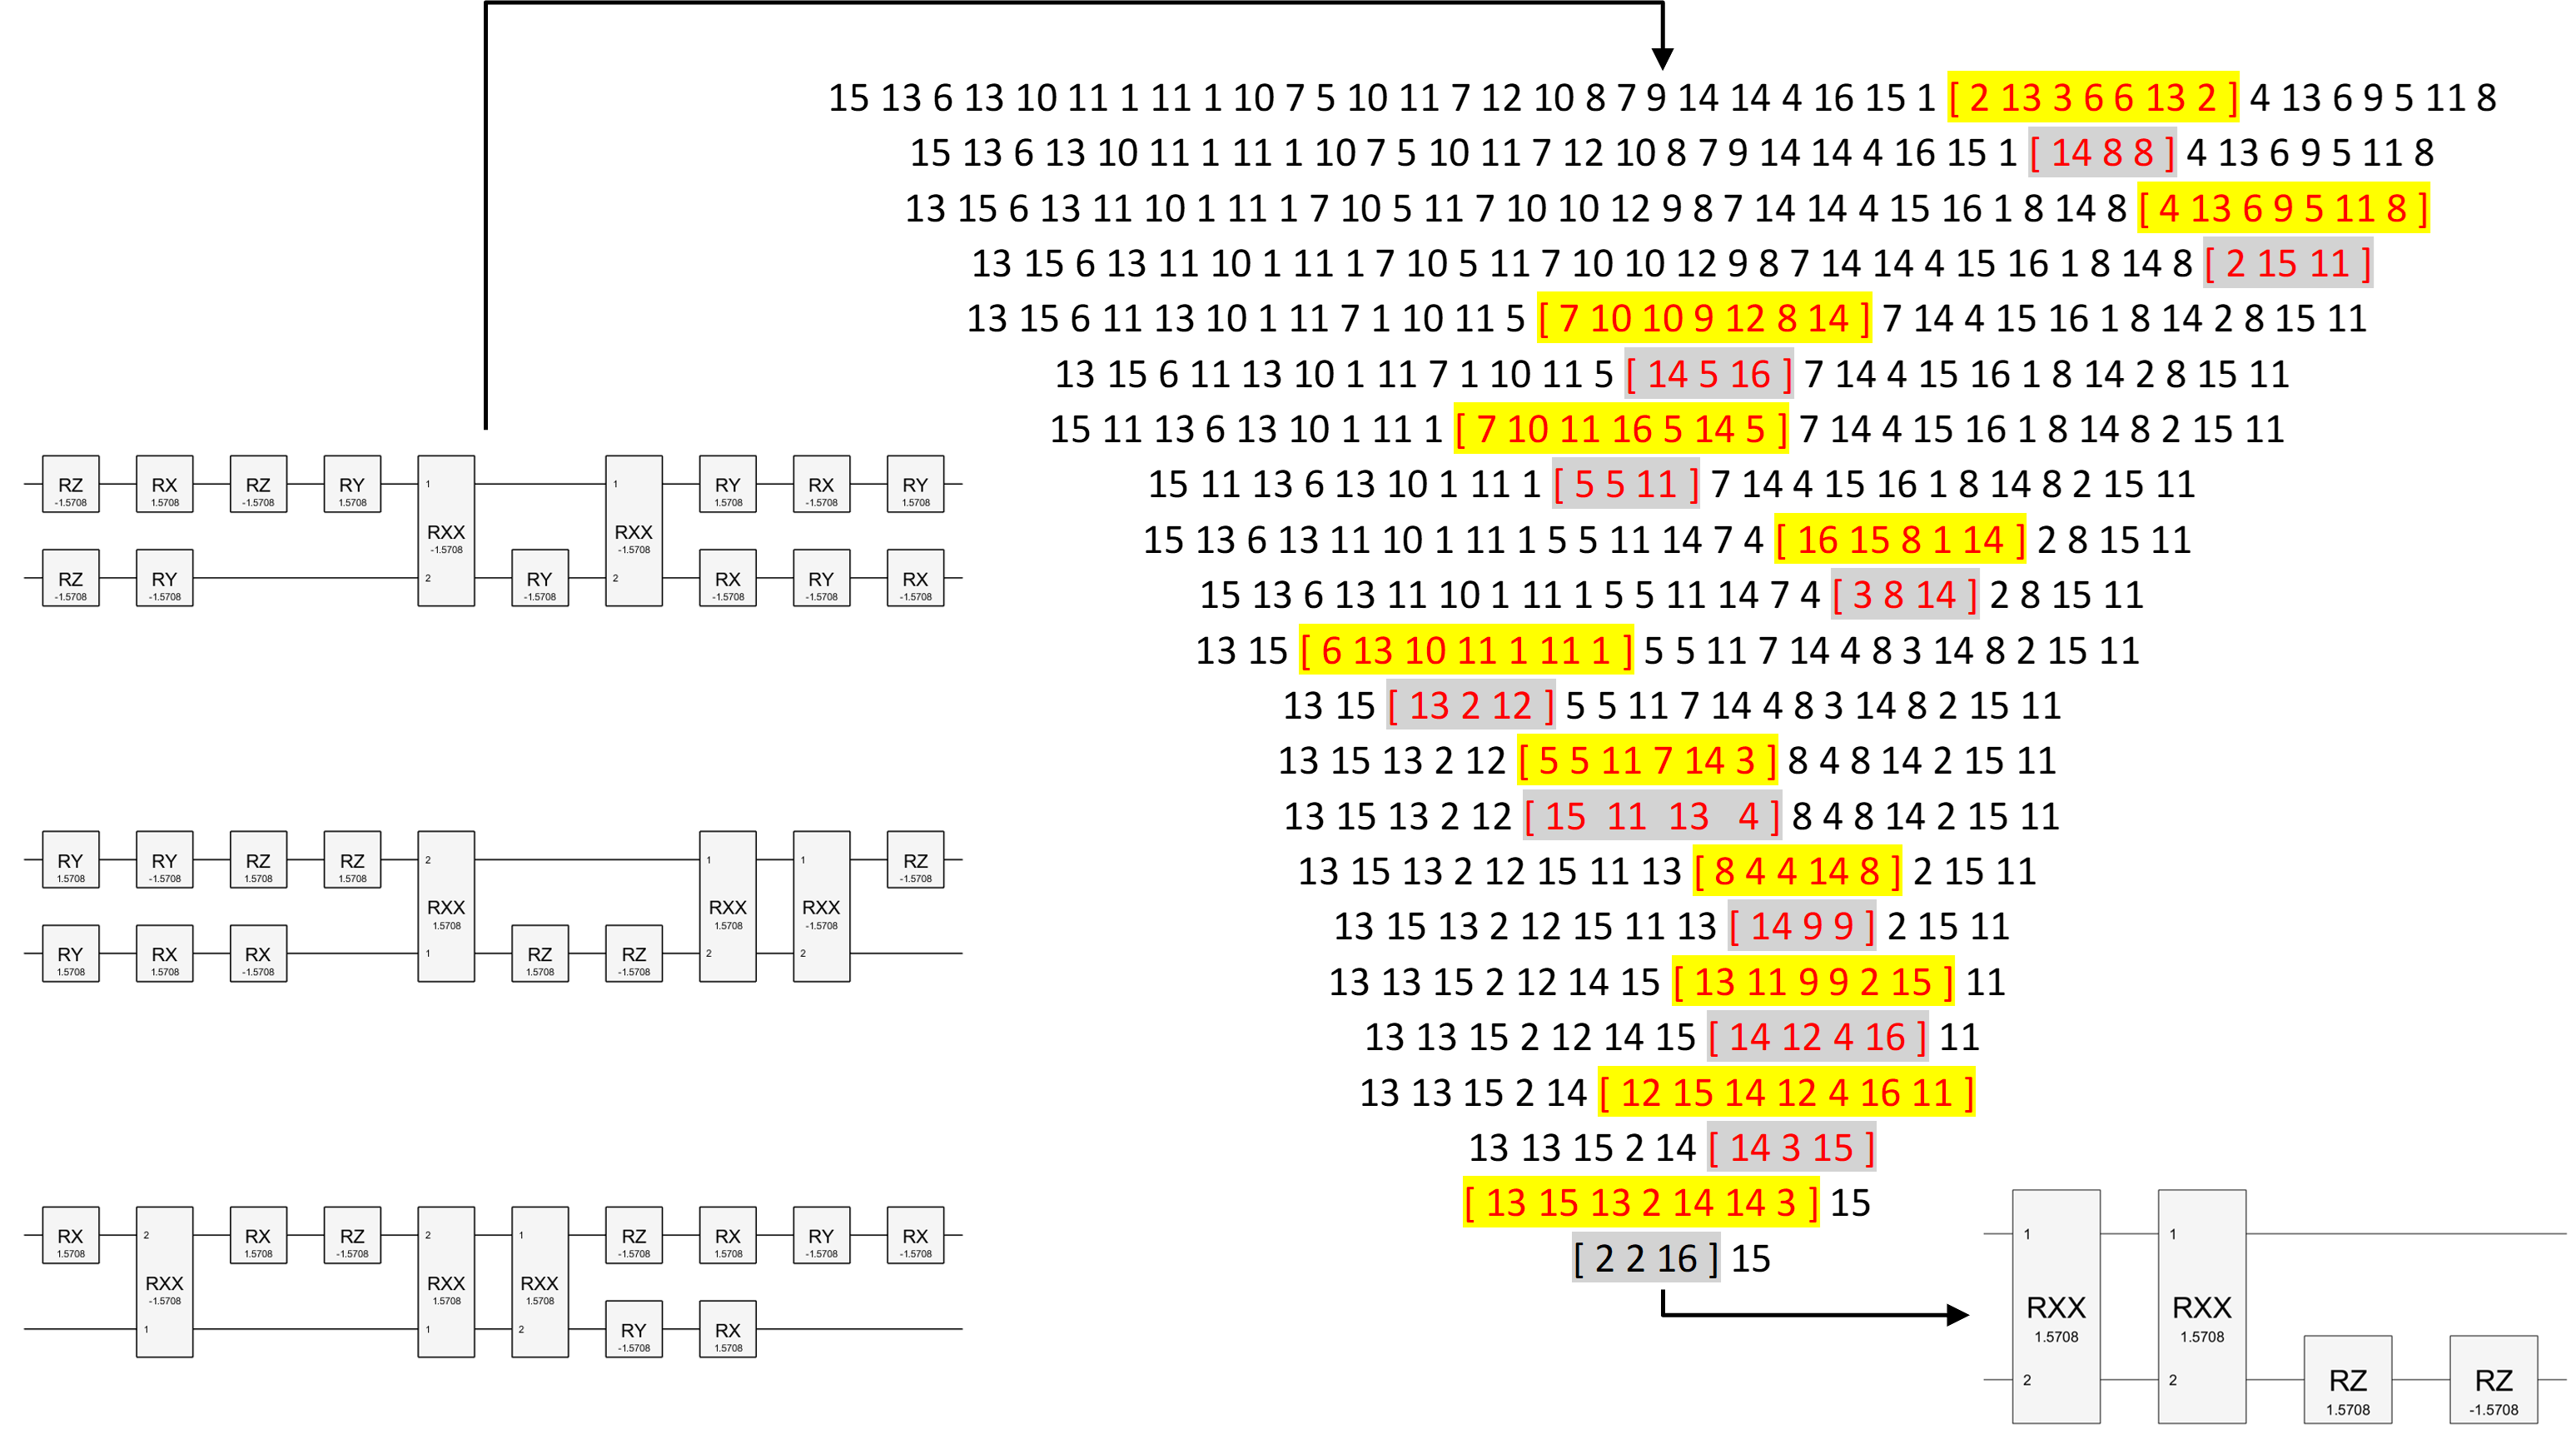
\includegraphics[width=0.85\textwidth]{CodeReduceTokens.png}
\caption{Paper Fig.~4: reducing a 40-gate 2-qubit circuit. Each line is the token chain after one replacement. Yellow =
selected block, grey = its shorter replacement on the next line. Bottom-right: final circuit.}
\end{figure}
\begin{careful}[title=Careful: the final circuit of Fig.~4 is not optimal (verified)]
The final circuit is $\RXX(\tfrac\pi2)\,\RXX(\tfrac\pi2)$ followed by $\RZ_2(\tfrac\pi2)\,\RZ_2(-\tfrac\pi2)$. The last two gates
multiply to the identity, so the true optimum is \textbf{2} gates. Two code details explain this. (i) \texttt{simplereduce.m}
loops \texttt{while(i<size-1)}, so it never checks the \emph{last} adjacent pair. (ii) The database deliberately omits the
root node (identity), so a block equal to the identity can never be ``looked up'' away. The loop stops at $<5$ gates, so it
stops here.
\end{careful}

\subsection{V2: compute-graph database retrieval}
Observation: blocks of 5--8 gates usually shrink to 2--4 gates, and every unitary with a $\le4$-gate circuit is in the
depth-4 compute graph. So build the graph once, store every node's unitary with its shortest path, and replace random
sampling with a lookup. A lookup is also a \emph{certificate}: if the block's unitary is not in the database among shorter
entries, the block is \emph{provably} irreducible to $\le d$ gates (with the chosen pool). The paper does the lookup by
comparing against all entries (a linear scan, about 4\,ms for 20k entries).

\begin{figure}[H]\centering
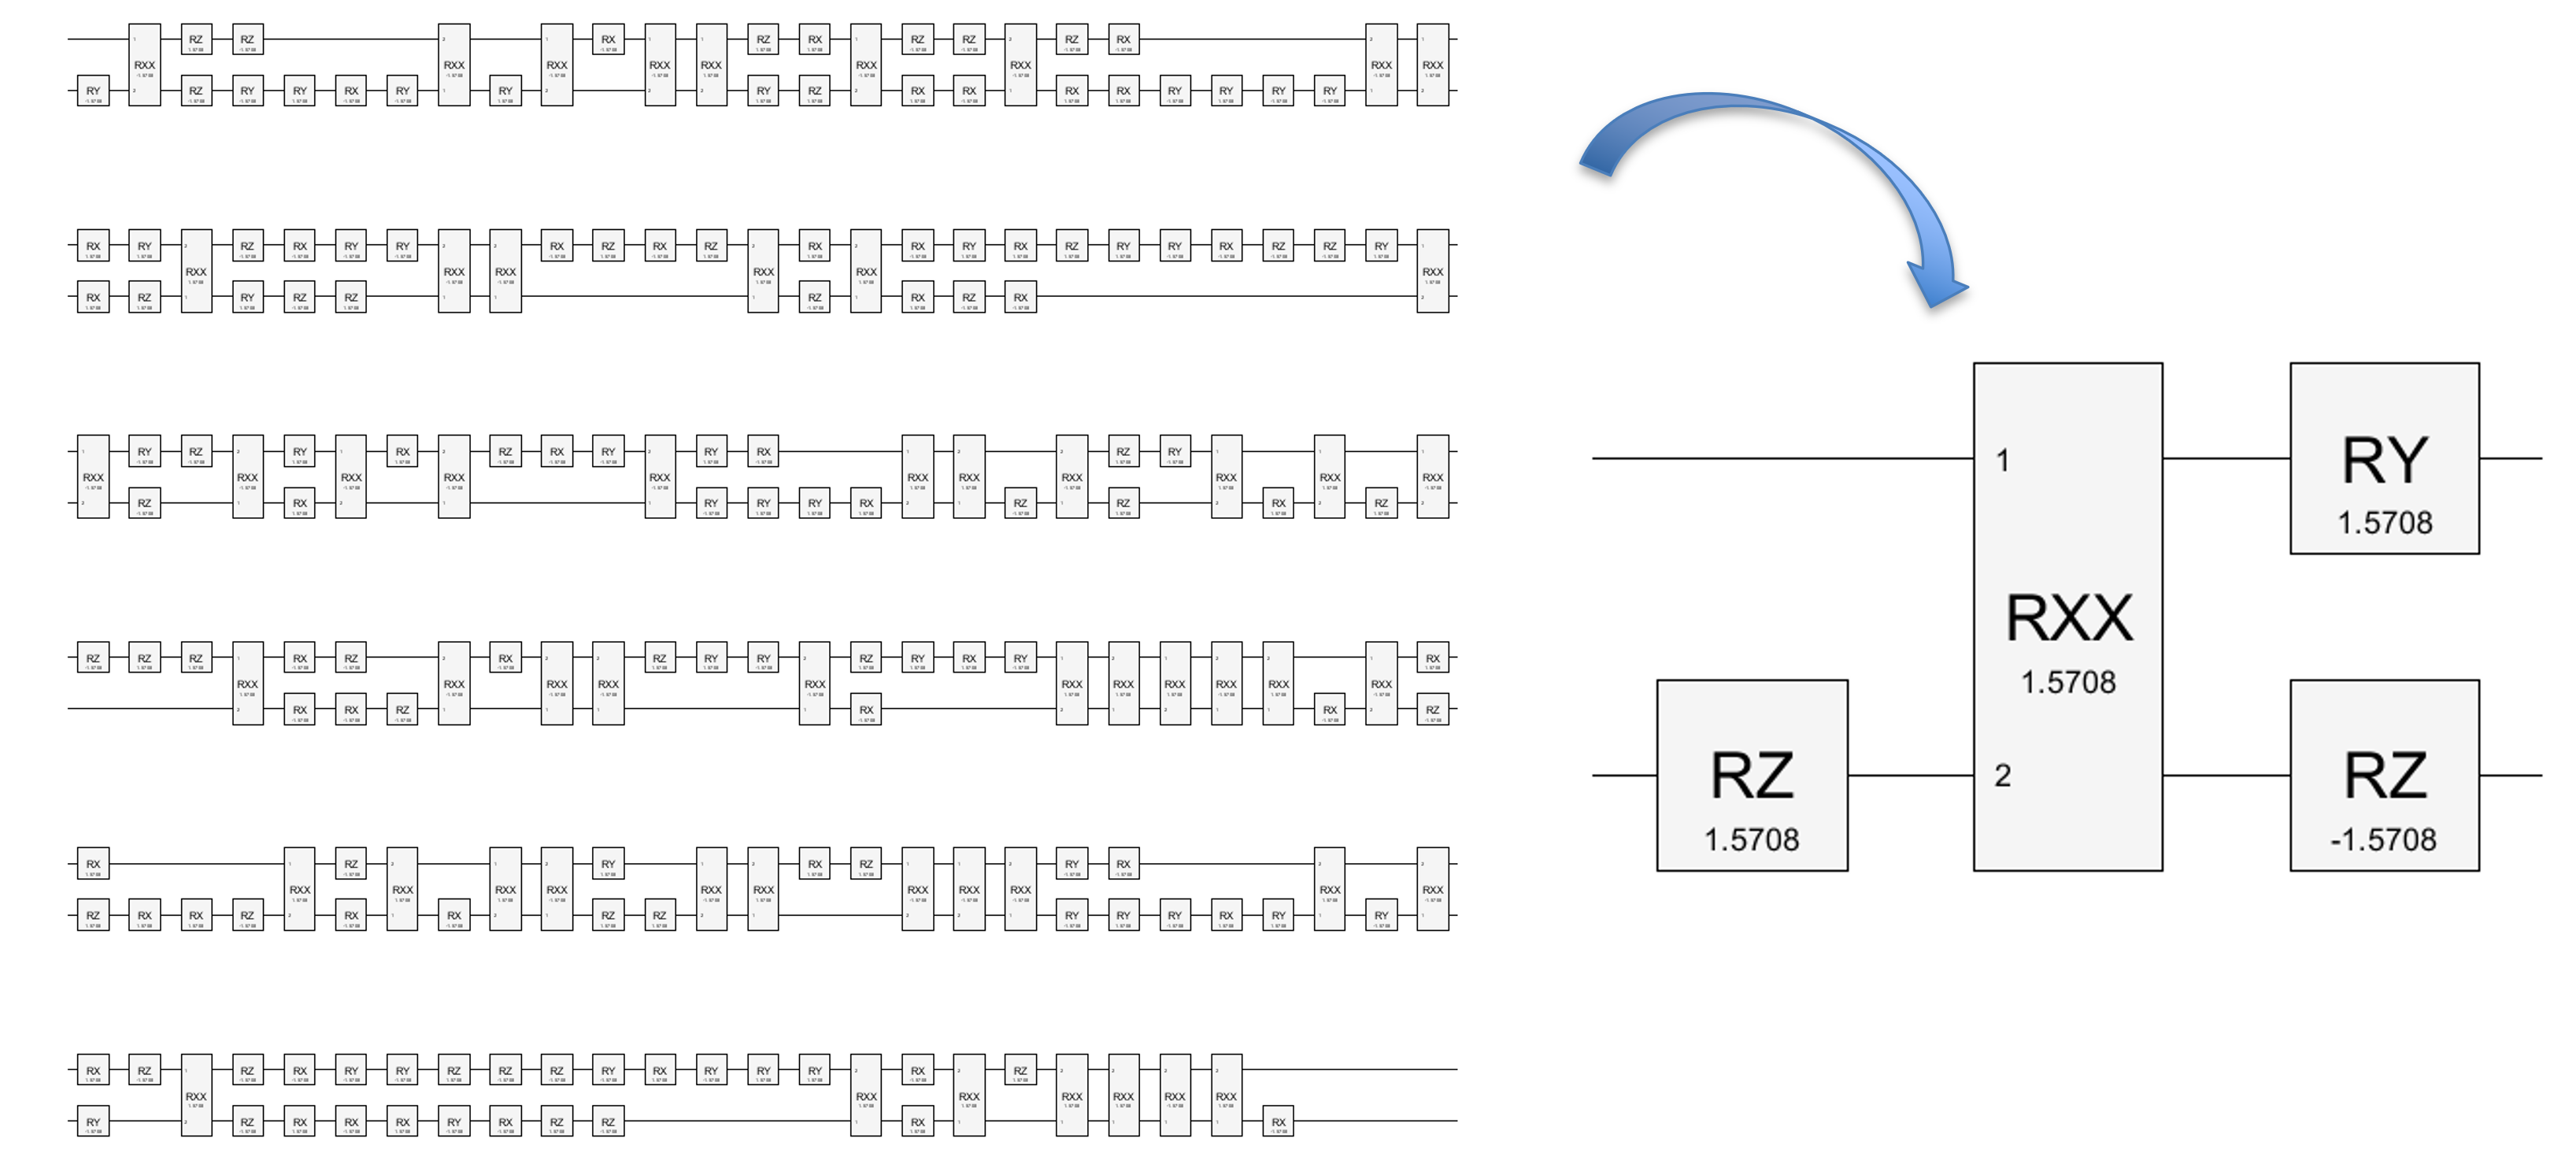
\includegraphics[width=0.8\textwidth]{In200Out4.png}
\caption{Paper Fig.~5 (\texttt{In200Out4}): a 200-gate input and its reduced form.}
\end{figure}

\subsection{V3: random-forest-gated lookup}\label{sec:v3}
A lookup costs $\approx4$\,ms, a forest call $\approx0.1$\,ms. If the forest rejects most irreducible blocks, the expensive lookup
is skipped. The paper trains the forest on compute-graph nodes (irreducible examples) and blocks that V2 reduced
(reducible examples).
\begin{careful}
Whether V3 is faster depends on the forest's \emph{recall}. Every reducible block it wrongly rejects is a lost opportunity
that must be re-found later. The paper reports neither precision nor recall. In our reproduction, at the default
threshold 0.5 the forest kept only 30\% of reducible blocks (held-out recall), and V3 became \emph{slower} than V2
(mean 172\,s vs.\ 46\,s). With threshold 0.2 (recall 92\%) it was the fastest variant (34\,s), matching the paper's ordering
(see the reproduction report). A hash table (\S8) makes the lookup itself $\sim$0.03\,ms, which
removes the reason for V3 altogether.
\end{careful}

%=====================================================================
\section{Paper \S IV: Experiments}
\subsection{Setting}
Most experiments use 2--3 qubits, because there every gate interacts with every other and reductions need more ``algebra''.
With many qubits, blocks are often on disjoint wires and easier.

\subsection{Convergence (Fig.~6) and statistics (Fig.~7, Table II)}
\begin{figure}[H]\centering
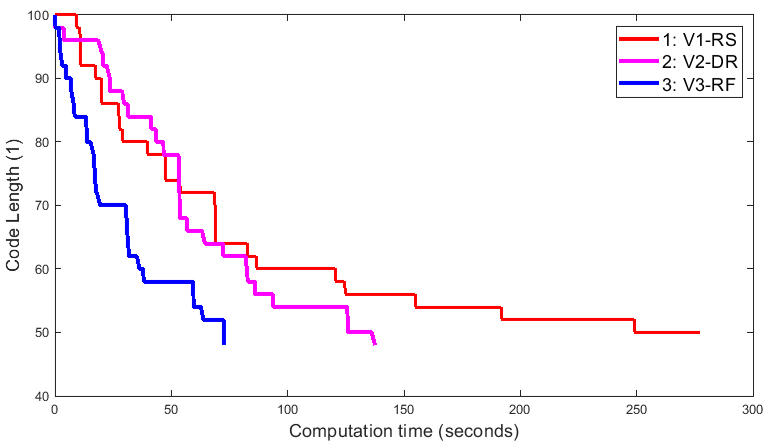
\includegraphics[width=0.55\textwidth]{ConvCurve3.png}
\caption{Paper Fig.~6 (\texttt{ConvCurve3}): circuit length vs.\ wall-clock time for one 100-gate circuit. Staircases:
each step down is one successful replacement; flat stretches are failed attempts. V3 (blue) reaches $\approx50$ first.}
\end{figure}
\begin{figure}[H]\centering
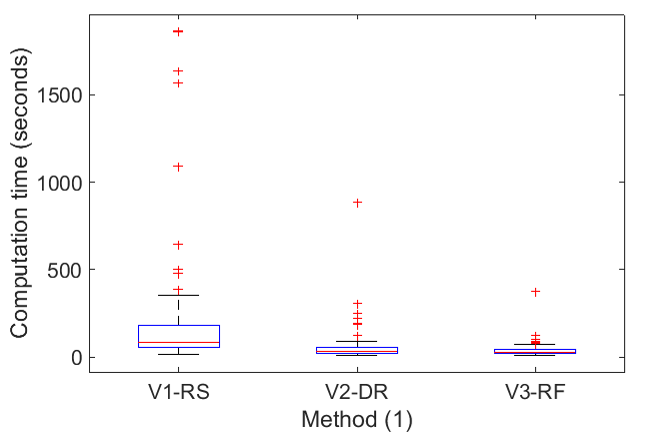
\includegraphics[width=0.48\textwidth]{Statistics2.png}
\caption{Paper Fig.~7: box plots of time-to-target over 100 random length-100 circuits. Red line = median, box = 25th--75th
percentile, whiskers = most extreme non-outliers, red crosses = outliers (MATLAB default: beyond $1.5\times$ the box height).}
\end{figure}
\begin{table}[H]\centering
\begin{tabular}{lccc}\toprule
(100 runs)&V1-RS&V2-DR&V3-RF\\\midrule
Mean (s)&199&55&38\\Std.\ dev.\ (s)&351.5&96.3&39.8\\\bottomrule
\end{tabular}
\caption{Paper Table II. Graph construction and forest training are excluded (``offline'').}
\end{table}
\begin{intuition}
\textbf{How to read it.} Std.\ dev.\ $>$ mean (V1, V2) means a heavy right tail: a few runs take extremely long, which
matches the outliers up to 1800\,s in the box plot. The ``target size'' and the qubit count are not stated; the curves
suggest about 50\% of the input length.
\end{intuition}

\subsection{Scalability: wire reduction (Fig.~8)}
\begin{figure}[H]\centering
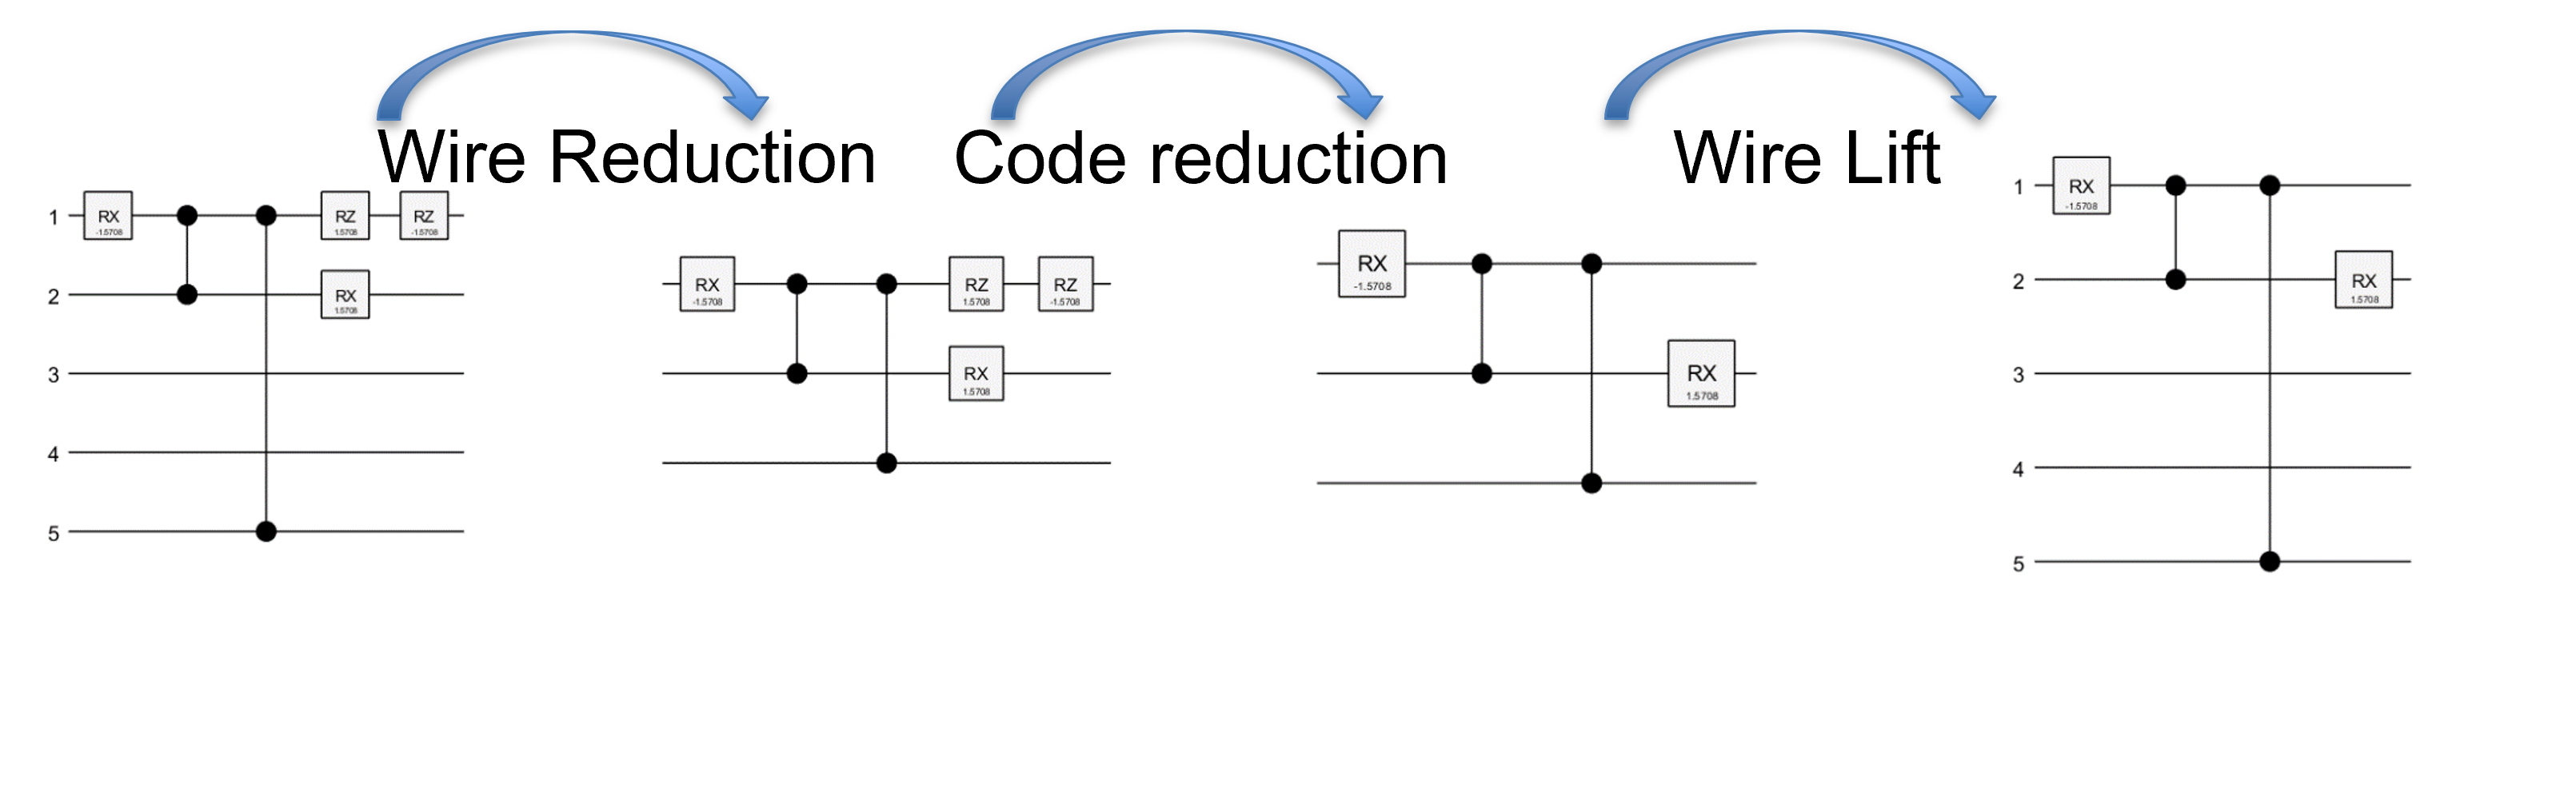
\includegraphics[width=0.8\textwidth]{ScalableOpt2.png}
\caption{Paper Fig.~8 (\texttt{ScalableOpt2}): a block on wires $\{1,2,5\}$ of a 5-qubit circuit is relabelled to wires
$\{1,2,3\}$ (``wire reduction''), reduced there, and mapped back (``wire lift'').}
\end{figure}
Because the database lives on 3 qubits, any block touching $\le3$ wires can be handled whatever the register size.
Disjoint blocks could be optimised in parallel. The compression rate drops for many qubits, because random gates rarely
interact.

\subsection{Comparison with Qiskit (Tables III--V)}
Qiskit's \texttt{transpile} at optimisation levels 1--3 (with the native basis) is compared with the paper's method on
one random circuit each.
\begin{table}[H]\centering\small
\begin{tabular}{l rrrr r}\toprule
\multicolumn{6}{c}{Table III: ion trap, 3 qubits}\\
Method&\#rx&\#ry&\#rz&\#rxx&\textbf{total}\\\midrule
original&86&88&86&40&300\\ qiskit L1&27&30&55&40&152\\ qiskit L2&22&41&83&35&181\\ qiskit L3&21&40&81&34&176\\
\textbf{ours}&\textbf{5}&\textbf{12}&\textbf{12}&\textbf{16}&\textbf{45}\\\bottomrule
\end{tabular}\hfill
\begin{tabular}{l rrr r}\toprule
\multicolumn{5}{c}{Table IV: IBM-style, 3 qubits}\\
Method&\#rx&\#rz&\#cz&\textbf{total}\\\midrule
original&115&118&67&300\\ qiskit L1&56&65&57&178\\ qiskit L2&62&49&42&153\\ qiskit L3&62&49&42&153\\
\textbf{ours}&\textbf{32}&\textbf{14}&\textbf{26}&\textbf{72}\\\bottomrule
\end{tabular}

\medskip
\begin{tabular}{l rrr r}\toprule
\multicolumn{5}{c}{Table V: IBM-style, 15 qubits}\\
Method&\#rx&\#rz&\#cz&\textbf{total}\\\midrule
original&96&91&313&500\\ qiskit L1&74&74&285&433\\ qiskit L2/L3&74&36&203&313\\
\textbf{ours}&\textbf{72}&\textbf{27}&\textbf{194}&\textbf{293}\\\bottomrule
\end{tabular}
\caption{Paper Tables III--V (totals added by us).}
\end{table}
\begin{intuition}
\textbf{Where do these circuits come from?} The gate proportions match drawing each token \emph{uniformly} from the
pool. 3-qubit ion pool: 3 of 21 gates are $\RXX$, so $300\cdot3/21\approx43$ (paper: 40). 15-qubit IBM pool: 105 $\CZ$ out of
$105+60$ gates, so $500\cdot0.64=318$ (paper: 313). So these are uniformly random native-gate circuits, not compiled algorithms.
\end{intuition}
\begin{careful}
\begin{itemize}[nosep]
\item One circuit per table, no repetitions and no error bars (the NJP version adds 100-circuit statistics, \S9).
\item The text says the IBM set is ``$\RX,\RY$ and CX'', but Tables IV--V report $\RX,\RZ,\CZ$.
\item Qiskit L2/L3 \emph{increase} \#rz relative to L1 in Table III. Qiskit's generic resynthesis does not know that the
  input is a Clifford over a 4-gate alphabet. A Clifford-aware baseline would be the fair comparison (\S10).
\item The 3-qubit results can be checked against the \emph{exact} optimum, because $|\mathcal C_3|$ is only $9.3\times10^7$
  (see the extension paper).
\item ``ours'' is much slower than Qiskit ($<1$\,s), which the authors acknowledge.
\end{itemize}
\end{careful}

\subsection{Hardware experiment (Fig.~9)}
A random 2-qubit circuit of length 40 (``long'') and its reduced 8-gate version (``short'') are transpiled by Qiskit for
two IBM Eagle r3 chips (127 qubits): \emph{Brisbane} (v1.1.33, EPLG 4.17\%) and \emph{Kyiv} (v1.20.12, EPLG 1.7\%). After
transpilation: long $\to$ 156 (Brisbane) / 148 (Kyiv) native operations; short $\to$ 34 / 32.
\begin{figure}[H]\centering
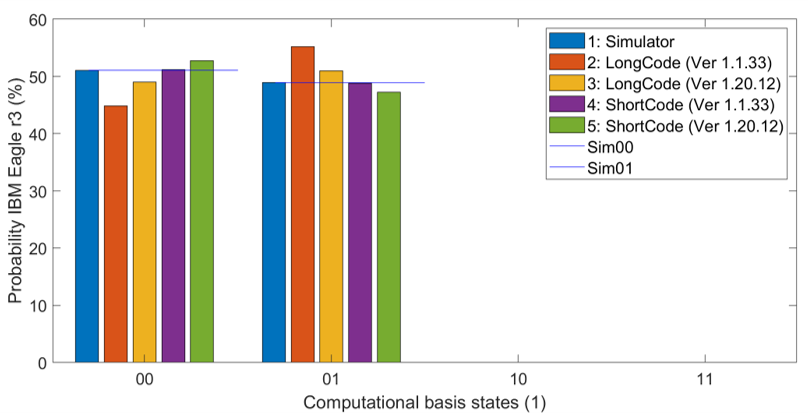
\includegraphics[width=0.6\textwidth]{QChipCompare1.png}
\caption{Paper Fig.~9: probabilities of outcomes 00, 01, 10, 11. Blue = ideal simulation ($\approx$51/49 on 00/01). The short
circuits (purple, green) lie closer to the simulation than the long ones (red, yellow). The newer chip (Kyiv) is closer than Brisbane.}
\end{figure}
\begin{careful}
\begin{itemize}[nosep]
\item One circuit, one run per chip; shot count and error bars not reported. The ideal output is almost a uniform mix
  of $\ket{00},\ket{01}$, a distribution that is not very sensitive to noise.
\item Qiskit's own level-3 transpiler re-synthesises any 2-qubit block into $\le3$ two-qubit gates. With level 3, the long
  and the short circuit would compile to essentially the same native circuit, so the gap shown depends on
  which transpiler level was used. The paper does not say which.
\item The comparison mixes two effects: circuit length and chip version.
\end{itemize}
\end{careful}

%=====================================================================
\section{Paper \S V: Summary and discussion}
The authors conclude that (i) local term replacement substantially reduces length; (ii) the database and the forest speed
it up; (iii) the method is slower than Qiskit and worthwhile when a block is reused many times; (iv) it can follow Qiskit as
a refinement step. They report that ZX-calculus simplification sometimes \emph{lengthened} their circuits after
re-extraction, and that IBM's AI transpiler does not support arbitrary gate sets. Future work: noise/duration-aware cost
functions, e.g.\ weighting two-qubit gates more than single-qubit gates.

%=====================================================================
\section{Mapping paper $\leftrightarrow$ code (``the code given'')}
The authors' MATLAB demo (\texttt{QCOptimDemo}) is linked only in the journal version, ref.~[38]:
\url{https://www.tnt.uni-hannover.de/en/staff/rosenhahn/QCOptimDemo.zip}. It needs MATLAB's \emph{Quantum Computing Support Package}
(\texttt{quantumCircuit}, \texttt{rxGate}, \texttt{getMatrix}). It is not Octave-compatible, so we ported it to Python.
\begin{center}\small
\begin{tabular}{p{4.2cm}p{10.6cm}}\toprule
File&Role\\\midrule
\texttt{QoperatorsIon1.m}&Builds the operator list for \texttt{dim} qubits: $\RXX_{ij}(\pi/2)$ for all $i<j$, then
$\RX,\RY,\RZ(\pm\pi/2)$ on each qubit. Also emits QASM strings.\\
\texttt{QoperatorsIon1M.m}&Same, but removes operators equal to the identity or to an earlier operator (database pool).\\
\texttt{FullQCGraphIOn3\_4.m}&Grows the compute graph (dim 3, depth 4) using a MATLAB \texttt{digraph}. New unitary $=$
\texttt{RM*R} (gate on the left, matching Eq.~1). Linear-scan duplicate check with tol $10^{-4}$. Saves
\texttt{Unitaries}, \texttt{OptOrder} (shortest paths), \texttt{OptLength} to \texttt{OptUnitDim3\_4.mat}.\\
\texttt{optimCodeGMode1DComp.m}&The optimiser (this is V2): random 300-gate 5-qubit circuit; commutation table;
loop {shuffle w.p.\ 0.7; sample block of 2--8 gates on $\le3$ wires; linear scan over DB entries shorter than the
block; replace; \texttt{simplereduce}}; stop at $<5$ gates (never reached in practice: runs until killed).\\
\texttt{compare.m}&Phase-insensitive distance (least-squares scale, spectral norm).\\
\texttt{simplereduce.m}&Deletes adjacent pairs whose product is the identity.\\
\texttt{ExtractWireMap.m}, \texttt{WireMapF.m}&Wire reduction/lift (relabel wires through \texttt{eval} of generated code).\\
\texttt{generateCodeNr.m}&Writes \texttt{longcode10.txt}/\texttt{shortcode10.txt} QASM after every improvement.\\\bottomrule
\end{tabular}
\end{center}
\begin{careful}[title=Code vs.\ paper discrepancies]
\begin{enumerate}[nosep]
\item Tolerance: paper $10^{-5}$; code $10^{-3}$ (optimiser) and $10^{-4}$ (graph builder).
\item Pools: Table I counts (14, 24) imply $\RXX(\pm\pi/2)$; the demo uses only $\RXX(+\pi/2)$ (13, 21 operators).
\item The database excludes the identity (\texttt{Dists>0}). Blocks equal to $I$ are only removable via \texttt{simplereduce}.
\item \texttt{simplereduce} skips the last pair and advances $i$ after a deletion, so it misses some cancellations (visible in Fig.~4).
\item V1 and V3 are not in the released code. Only V2 is.
\item The graph builder recomputes BFS distances only with probability 0.3 per step, so its ``depth'' is approximate during
  growth. Our exact BFS gives identical counts for Table I, so this has no effect on the reported numbers.
\end{enumerate}
\end{careful}

%=====================================================================
\section{What changed in the published version (New J.\ Phys.\ 27, 104509, 2025)}
The journal version keeps Sections I--III and adds (i) BQSKit levels 2--4 as baselines, (ii) new single-circuit tables at
4 qubits (ion trap) and 6 qubits (IBM), and (iii) 100-circuit statistics (4 qubits, length 300):
\begin{center}\small
\begin{tabular}{lrrrr|rrr}\toprule
&\multicolumn{4}{c|}{Ion trap, 4q, mean (std)}&\multicolumn{3}{c}{IBM-style, 4q, mean (std)}\\
Method&rx&ry&rz&rxx&rx&rz&cz\\\midrule
Input&78(7)&83(8)&78(7)&59(7)&108(9)&109(8)&82(8)\\
Qiskit L3&33(6)&49(5)&66(9)&56(8)&59(5)&39(4)&51(6)\\
BQSKit L4&40(7)&0(0)&58(19)&28(4)&56(10)&75(15)&37(7)\\
\textbf{Ours}&10(3)&29(6)&29(5)&43(8)&45(6)&19(4)&43(6)\\\bottomrule
\end{tabular}
\end{center}
Note that BQSKit L4 beats ``ours'' on two-qubit gates ($\RXX$: 28 vs.\ 43; $\CZ$: 37 vs.\ 43), the gates that dominate
hardware error. The journal text reportedly uses angle grids including $\pm\pi/4$, which would make the gate set non-Clifford.
The released code uses only $\pm\pi/2$.

%=====================================================================
\section{Critical assessment}
\textbf{Strengths.} Simple, gate-set-agnostic and easy to implement. Every replacement is exact (no approximation), so
correctness is easy to check. The database turns search into lookup and certifies irreducibility. Wire reduction is a
clean way to use a small database on large registers. The idea of composing with existing transpilers is sensible.

\textbf{Weaknesses} (developed fully in the accompanying extension paper):
\begin{enumerate}[nosep]
\item \textbf{The Clifford structure is ignored.} All gates are Clifford. The search space is a finite group with
  exact $O(n^2)$-bit fingerprints and known optimal-synthesis results (complete for $n\le3$). Global optima can be computed exactly
  for the paper's 2- and 3-qubit experiments, so the paper's results can be scored against ground truth, but it never does.
\item \textbf{Floating-point identification} with ad hoc tolerances, and an $O(N)$ linear scan where a hash lookup is $O(1)$. That alone
  makes V3's motivation disappear.
\item \textbf{Locality.} Contiguous windows of $\le 8$ tokens in one linear order, explored by random commuting swaps. There is no
  guarantee of local optimality and no notion of convergence. The right object is the circuit DAG (trace monoid).
\item \textbf{Evaluation.} Single random circuits for Tables III--V. Unspecified qubit counts and targets for Table II. Wall-clock
  time across MATLAB vs.\ an unspecified machine. No Clifford-aware, ZX, TKET, Quarl/Quartz/QUESO, or exact baselines (the closest prior
  work, Quartz [Xu et al., PLDI 2022], also builds an equivalence-class database by enumeration).
\item \textbf{Cost function} is total gate count. Two-qubit gate count, depth, and fidelity are not optimised.
\item \textbf{Hardware evidence} rests on a single 2-qubit circuit with no uncertainty quantification and an unspecified transpiler level.
\item \textbf{Code} omits V1/V3, and has the bugs above.
\end{enumerate}

%=====================================================================
\section{Does it reproduce? (summary of our reproduction)}
We ported the authors' MATLAB code line by line to Python and re-ran every experiment. Details are in
\texttt{manuscripts/reproduction/reproduction\_report.pdf}.
\begin{center}\small
\begin{tabular}{p{4.0cm}p{2.3cm}p{8.4cm}}\toprule
Claim&Verdict&What we found\\\midrule
Table I (graph sizes)&reproduced&All node and edge counts identical.\\
Fig.~1, Fig.~4&reproduced&Equivalences hold. But Fig.~4's output (4 gates) has optimum 2, because of a code bug.\\
Table II / Figs.~6--7&partly&V1 254\,s, V2 46\,s, V3 172\,s (threshold 0.5) or 34\,s (threshold 0.2). The paper's ordering needs a tuned
forest threshold; the forest's recall at 0.5 is only 30\%.\\
Table III (ion trap, 3q)&reproduced&47.1 gates (paper 45), but only with the larger 24-op depth-5 database. The demo database gives $\approx76$.\\
Table IV (IBM-style, 3q)&reproduced&36.8 gates (paper 72).\\
Table V (15q)&not reproduced&The method ties a modern Qiskit 2.5 (336 vs.\ 332 gates); the paper reports 293 vs.\ 313.\\
NJP 4q statistics&reproduced&78.8 / 76.0 gates (published 111 / 107). Qiskit L3 165 / 141.\\
Fig.~9 (hardware)&partly&Noisy simulation of the same two chips, 30 circuits: the short circuit wins at transpiler levels 0/1. The
advantage disappears at level 3.\\\bottomrule
\end{tabular}
\end{center}
\textbf{How good is ``good''?} Because all gates are Clifford we could compute the \emph{exact} optimum of every 3-qubit circuit.
On the Table III/IV setting the optimum is 10.5 (ion trap) and 12.3 (IBM-style) gates, so the paper's method is 4.5$\times$ and
3.0$\times$ longer than necessary. An exact-window optimiser reaches the optimum in about 0.2\,s. See the extension paper.

%=====================================================================
\section{Questions you may be asked (with answers)}
\begin{enumerate}[leftmargin=*]
\item \emph{Why compare unitaries only up to a global phase?} Because $e^{i\varphi}U$ and $U$ give identical measurement
  statistics for every input. Phase is unobservable.
\item \emph{Why is the compute graph much smaller than $|\mathcal{OP}|^d$?} Different gate strings give the same unitary
  (commutations, inverses, relations such as $\RX(\tfrac\pi2)^4\simeq I$), so paths merge.
  For a finite group, the graph eventually stops growing.
\item \emph{What does the database lookup guarantee?} If no shorter entry exists, the block cannot be shortened to $\le d$ gates from
  that pool. It is a certificate of local irreducibility.
\item \emph{Why does V3 help, and when does it hurt?} It replaces a 4\,ms lookup with a 0.1\,ms prediction, but a false negative throws
  away a real reduction. With low recall the run gets slower.
\item \emph{Why do Qiskit L2/L3 sometimes give more single-qubit gates than L1?} Generic resynthesis into Euler angles,
  plus translation of each to the restricted $\pm\pi/2$ alphabet, can expand single-qubit runs.
\item \emph{How does the method scale to 15 qubits?} By wire reduction. Only blocks on $\le3$ wires are optimised, with the 3-qubit database.
\item \emph{Is the output optimal?} No. It is a local optimum under random windows. For 2 qubits the exact optimum is a single lookup in a
  11,520-entry table. The paper's Fig.~4 output (4 gates) has an optimum of 2.
\item \emph{What is a Clifford gate, and why does it matter here?} See \S\ref{sec:clifford}. It turns the problem into exact
  combinatorics on a finite group.
\end{enumerate}

\vfill
{\small\textit{Companion material:} \texttt{qcr/} and \texttt{experiments/} contain the Python port and all experiments
(\texttt{manuscripts/reproduction/reproduction\_report.pdf}); \texttt{manuscripts/extension/extension\_paper.pdf} contains the follow-up research paper.}
\end{document}
